\documentclass[a4paper,11pt]{article}

\usepackage{amsmath}
\usepackage{listings}
%package to fix images where they are defined with option H
\usepackage{float}

% Paquetes para matemáticas:
\usepackage{amsmath, amsthm, amssymb, amsfonts, amscd} % Teoremas, fuentes y símbolos.
\usepackage{tikz-cd} % para diagramas conmutativos
% for writing inference rules
\usepackage{proof}
% for quotes
\usepackage[autostyle]{csquotes}  
 % Nuevo estilo para definiciones
 \newtheoremstyle{definition-style} % Nombre del estilo
 {5pt}                % Espacio por encima
 {0pt}                % Espacio por debajo
 {}                   % Fuente del cuerpo
 {}                   % Identación: vacío= sin identación, \parindent = identación del parráfo
 {\bf}                % Fuente para la cabecera
 {.}                  % Puntuación tras la cabecera
 {\newline}               % Espacio tras la cabecera: { } = espacio usal entre palabras, \newline = nueva línea
 {}                   % Especificación de la cabecera (si se deja vaía implica 'normal')

 % Nuevo estilo para teoremas
 \newtheoremstyle{theorem-style} % Nombre del estilo
 {5pt}                % Espacio por encima
 {0pt}                % Espacio por debajo
 {\itshape}           % Fuente del cuerpo
 {}                   % Identación: vacío= sin identación, \parindent = identación del parráfo
 {\bf}                % Fuente para la cabecera
 {.}                  % Puntuación tras la cabecera
 {\newline}               % Espacio tras la cabecera: { } = espacio usal entre palabras, \newline = nueva línea
 {}                   % Especificación de la cabecera (si se deja vaía implica 'normal')

 % Nuevo estilo para ejemplos y ejercicios
 \newtheoremstyle{example-style} % Nombre del estilo
 {5pt}                % Espacio por encima
 {0pt}                % Espacio por debajo
 {}                   % Fuente del cuerpo
 {}                   % Identación: vacío= sin identación, \parindent = identación del parráfo
 {\scshape}                % Fuente para la cabecera
 {:}                  % Puntuación tras la cabecera
 {.5em}               % Espacio tras la cabecera: { } = espacio usal entre palabras, \newline = nueva línea
 {}                   % Especificación de la cabecera (si se deja vaía implica 'normal')

 % Teoremas:
 \theoremstyle{theorem-style}  % Otras posibilidades: plain (por defecto), definition, remark
 \newtheorem{theorem}{Theorem}[section]  
 \newtheorem{lemma}{Lemma}[section]
 \newtheorem{corollary}{Corollary}[section]  
 \newtheorem{exercise}{Exercise}[section]  

 % Definiciones, notas, conjeturas
 \theoremstyle{definition-style}
 \newtheorem{definition}{Definition}[section]
  
\usepackage[]{algorithm2e}  
\usepackage{algorithmic}
\usepackage{url}
\usepackage[french,british]{babel}
\lstdefinestyle{freefempp}{
  language=C++,
  basicstyle=\footnotesize\ttfamily,
  commentstyle=\itshape\color{violet},
  identifierstyle=\color{blue},
  morekeywords={ border, buildmesh, cos, dx, dy, fespace, fill, func,
    int2d, label, mesh, on, pi, plot, problem, sin, real, x, y},
  % float,
  frame=single,
  numbers=left
}
\lstset{style=freefempp}
\begin{document}
\section{Interaction paradigms}
The term Human-Computer Interaction (HCI) refers to the study of interaction between humans and computers. The scientific field of HCI has seen considerable advancements in the last 30 years, especially since the publication of Card, Moran and Newell’s Psychology of Human Computer Interaction in 1983. Most of the research efforts in HCI attempt to make use of human skills and abilities that are naturally developed by leading a life in this physical world. One can classify different paradigms of interaction that take place between humans and computers:

\subsection{Command lines}

Initial interfaces were command-line interfaces where a user sits in front of a terminal screen, and enters a line specific command to perform specific tasks and wait for a reply. Only a part of the terminal screen real estate was used. Some of the concepts that were introduced were the concept of infinite loop (prompt), the immediate execution of commands (enter), a syntax allowing obligatory or optional parameters, the maintenance of a history of commands and the introduction of keyboard short-cuts. They were further improved with the introduction of textual interfaces that made use of the entire terminal screen.

\subsection{WIMP (Windows, icons, menus and pointers)}

The WIMP paradigm relies on Windows, Icons, Menus and Pointers to interact with the user.  

\begin{itemize}
\item A window runs a self-contained program, isolated from other programs that (if in a multi-programmed operating system) run at the same time in other windows.
\item An icon acts as a shortcut to an action the computer performs (e.g., execute a program or task).
\item A menu is a text or icon-based selection system that selects and executes programs or tasks.
\item The pointer is an on-screen symbol that represents movement of a physical device that the user controls to select icons, data elements, etc.
\end{itemize}

Post-WIMP comprises work on user interfaces, mostly graphical user interfaces, which attempt to go beyond this paradigm.

The reason WIMP interfaces have become so prevalent is that they are very good at abstracting work-spaces, documents and their actions. Their analogous paradigm to documents as paper sheets or folders makes WIMP interfaces easy to introduce to other users. 

However, WIMP interfaces are not optimal for working with complex tasks such as showing 3D models (computer-aided design), working on large amounts of data simultaneously (interactive games) or simply portraying an interaction for which there is no defined standard widget. WIMPs are usually pixel-hungry, so given limited screen real estate they can distract attention from the task at hand.  

\subsection{Direct manipulation interface}

It was introduced in the context of the creation of office applications and the desktop metaphor. It involves continuous representation of objects providing actions that are rapid, reversible, incremental and with feedback. These actions should correspond to manipulation of physical objects. Example: resizing a graphical shape by dragging its corners or edges with a mouse or doing a drag-n-drop to delete a file.

Benefits: can make it easier for a user to learn and use an interface, having rapid, incremental feedback allows a user to make fewer errors and complete tasks in less time.

\subsection{Form filling}

It is preferred for bureaucratic and routine tasks. Introduces the notion of obligatory, optional or conditional fields, the notion of unfolding menus, the guide of the user during the process and the use of short-cuts. It allows the automatic verification of inputs. Example: online reservation of a flight. 

\subsection{Experiment with the four previous paradigms}

The experiment that can be found \url{http://cs211labs.epfl.ch} does a simulation of the purchase of five tickets in each of the four previous interaction modes. The conclusion is that the best paradigm depends on the task, the user and the details of the design. 

Depending of the degree of use of the tool we can have a beginner, an intermediate or an expert user. A beginner user will only retain the aspects of the task that he needs to know in the real world without using a computer. The intermediate user will also know more advanced features that help to do the translation of the task from the real world to the computer. Finally, the expert user master aspects inherent to the computer program itself that don't have to do with the task itself.

Example: if we take OpenOffice Word, the beginner should know that he needs an index, an introduction and a body for writing an essay. The intermediate user will know that in order to structure the body of his essay he needs to structure the text in paragraphs and can set the parameters to separate paragraphs and set its style. Finally, the expert user will master where are the options set in the application or what is the formal languages used for specific actions.


\subsection{Virtual reality}

Computer interactive simulation using sound and visual effects corresponding to real, imaginary or semi-imaginary environments.

Examples: Minecraft (characters represented by avatars although the world is not real), eye surgery learning.

An interactive computer simulation is immersive if the user receives similar stimulus to the ones he would receive in the environment that is being simulated. The stimulus can be in all senses: sight, smell, touch or sound.

Examples: a cave automatic virtual environment (CAVE) is an immersive virtual reality environment where video projectors are directed to between three and six of the walls of a room-sized cube. CAVE is typically a video theater situated within a larger room. The user wears 3D glasses inside the CAVE to see 3D graphics generated by it. People using the CAVE can see objects apparently floating in the air, and can walk around them, getting a proper view of what they would look like in reality. A CAVE user's movements are tracked by the sensors typically attached to the 3D glasses and the video continually adjusts to retain the viewers perspective.

A question remains to be answered. Do these virtual reality experiences really influence the users as the real world does. Several experiments have been conducted in this sense, measuring physiological and cognitive responses. For instance, virtual  reality  users  hearts  have  pumped intensely  while  crossing  a  virtual pit (walking through a piece of wood surrounded by virtual cliffs. 

Difference haptics (related to the touch sense) devices has been implemented. The give the sensation of touch by applying forces (force feedback) or vibrations to the movements of users. This needs the presence of sensors for measuring the forces applied by the user. The user can then feel the specific resistance, elasticity or rugosity of the surface

Applications:  surgery simulations, bass shakers vibrations in cinemas. 

A particularly interesting applications is a data glove or wired glove. It is an input device for human-computer interaction worn like a glove. Various sensor technologies are used to capture physical data such as bending of fingers. Often a motion tracker, such as a magnetic tracking device or inertial tracking device, is attached to capture the global position/rotation data of the glove. 

These movements are then interpreted by the software that accompanies the glove, so any one movement can mean any number of things. Gestures can then be categorized into useful information, such as to recognize sign language or other symbolic functions.

Expensive high-end wired gloves can also provide haptic feedback, which is a simulation of the sense of touch. This allows a wired glove to also be used as an output device. Wired gloves are often used in virtual reality environments and to mimic human hand movement by robots.

\subsection{Tangible interaction}

Tangible Interaction has come to be the 'umbrella term' used to describe a set of related research and design approaches which have emerged in several disciplines. It covers user interfaces and interaction approaches that emphasize:

\begin{itemize}
\item tangibility and materiality of the interface which is then connected with sensors with the computer. This sensors can be in the form of cameras, touch-tables or RFID.
\item the objects employed are specific to the task at hand which can be the visit to a museum to learn about an specific topic or directed to children to learn programming. It is very usual that this physical environments are thought to be multi-user to enhance teamwork. 
\end{itemize}

\subsection{Augmented reality}

Augmented reality (AR) , is a live direct or indirect view of a physical, real-world environment whose elements are augmented by computer-generated sensory input such as sound, video, graphics or GPS data. Augmented reality enhances one’s current perception of reality, whereas in contrast, virtual reality replaces the real world with a simulated one. Augmentation techniques are typically performed in real-time, that is, there are time limits that must be met, and in a semantic context with the addition to the environmental elements of overlaying supplemental information like scores over a live video feed of a sporting event.

There are several hardware instruments that can be used to this goal. Using transparencies such as glasses or projections. We can even have interactive surfaces where we should ask ourselves whether is better to project from the upside or from the downside. A special characteristic of this surfaces is whether they are multi-touch or not. Multi-touch means that we can recognize the presence of more than one or more than two points of contact with the surface

\subsection{Difference between virtual reality and augmented reality}

Virtual reality offers a digital recreation of a real life setting, while augmented reality delivers virtual elements as an overlay to the real world. 

\subsection{Voice command devices}

These are interfaces that allow the user to communicate using its voice with the computer. A popular system for this is Siri. However, there is still a lot to do in human voice recognition to generalize these tools.  The level of precision depends on factors like the size of the vocabulary of the user, the environmental noise, the time that a particular user has been using it since Siri claims that it can learn with time or certain others semantic problems. There are also certain challenges in its usability.

\subsection{Gesture control}

This interface is based in the recognition of human gestures. In EPFL, reseracher Frédéric Kaplan has developed such a system to simulate tennis games. Microsoft Kinect is also an examples. It enables users to control and interact with their console/computer without the need for a game controller, through a natural user interface using gestures and spoken commands.

\subsection{Brain–computer interface}

These interfaces allow the communication of the user's brain activity to the computer. In EPFL, researchers have obtained results controlling a wheel-chair. The thoughts of the user activate specific brain patterns that are recorded by electroencephalography (EEG) using a helmet with electrodes. These patterns are then interpreted by a computer that transmits a command to the chair. Interestingly, it takes some time to the user of this systems to adapt their thoughts to the machines they use. It is a process of mutual apprenticeship between human and machine.

\subsection{Bionic interfaces}

Bionics is the application of biological methods and systems found in nature to the study and design of engineering systems and modern technology. Therefore a bionic interface is an interface that profits of this knowledge to communicate the user and the computer.

An interesting experiment was carried out in EPFL by the team of Silvestro Mícera to make a bionic hand with which patients could adjust their force to take objects and identify their shape and texture. The prosthesis contained some sensors capable of reacting to the tension of artificial tendons at translating them into electric impulses. This electric signals could then be transmitted to the actual external nerves of the patient arm.

\subsection{Wearables interfaces}

Wearable technology or wearables are electronic devices with microcontrollers that can be worn on the body as implants or accessories. The designs often incorporate practical functions and features.

This can be used for instance for sousveillance, which is the recording of an activity by a participant in it by means of wearing certain objects. It has also been used in the fashion industry. CuteCircuit was the first fashion company offering smart textile-based garments that create an emotional experience for their wearers using smart textiles and micro electronics.

\subsection{Interaction ambient}

The notion of ambient devices revolves around core concept of immediate access to information. The original developers of the idea (HYATT, ROSE, 2002) state that in the majority of cases an ambient device is designed to provide support to people in carrying out their everyday activities in an easy and natural way. An average person living in a modern society is being overloaded with abundance of information on a daily basis. Through the introduction of ambient devices into their day-to-day routine an individual gains an opportunity to decrease the amount of effort to process incoming data, thus rendering self more informed and productive (ROSE, 2002).

The key issue lies within taking Internet-based content (e.g. traffic congestion, weather condition, stock market quotes) and mapping it into a single, usually one-dimensional spectrum (e.g. angle, colour). According to one of the concept originators David L. Rose this way the data is represented to an end user seamlessly, and its procurement requires an insignificant amount of cognitive load.

One of the examples of the ambient device technology is Ambient Orb, introduced by Ambient Devices in 2002 (KIRSNER, 2002). The device itself was a glowing sphere which was continuously displaying data through perpetual changes in colour. Ambient Orb was customizable in terms of content and its subsequent visual representation. For instance, when the device was set to monitor a particular stock market index (e.g. NASDAQ), the Orb glowed green/red to represent the upward/downward movement of the stock prices; alternatively, it turned amber when the index is unchanged. Nabeel Hyatt stated that the device was marketed as an interior design item with additional functionality.

\subsection{Final thoughts}

Often, interfaces are said to be intuitive. However, we all have to learn how things work. The fact that we think that an interface is intuitive is more related with the fact hat we forget that we have learnt it. To properly asses the quality of a good interface one has to measure:

\begin{itemize}
\item the learning curve
\item the time needed to complete tasks
\item the number of errors
\item the user satisfaction
\end{itemize}

\subsection{Exercises}

\begin{exercise}
Suppose a website for reserving plane tickets. Classify the following knowledges into the different categories:
\end{exercise}
\begin{itemize}
\item If a user waits very long before confirming his choice the session is stopped and he has to restart all the process. (related to the computer translation)
\item A user has to enter the departure and arrival airports that are in the scope of the company's flights. (related to the computer translation)
\item Each airport of the world has a code name in three letters. For instance, GVA for Geneva. (related to the task)
\item In Swiss.com if the user wants to reserve a ticket in business class, he has to click on "more options" in the first dialogue window. (related to syntax)
\item I can order the possible flights in terms of the number of layovers or the price. (related to the computer translation)
\end{itemize}

\begin{exercise}
A software program for 3D rendering offers multiple functionalities to architects. What interaction paradigm is the most appropiate for the listed tasks. (It is possible to have several).
\end{exercise}
\begin{itemize}
\item Position a numeric image of the furniture and the equipment in the interior of the future kitchen. (direct manipulation)
\item position a numeric image of the future house on a real image of the ground to understand ints integration in the landscape. (augmented reality)
\item Make the the listing of the required windows for each room of the house. (form filling)
\item Propose to the clients an immersive visit in their future house. (virtual reality)
\end{itemize}


\section{Introduction to Computer Graphics}
Although computer graphics is a vast field that encompasses almost any graphical aspect, we are mainly 
interested in the generation of images of 3-dimensional scenes. Computer imagery has applications for film 
special effects, simulation and training, games, medical imagery, flying logos, etc.

Computer  graphics  relies  on  an  internal \textbf{model} (modeling) of  the  scene, that  is,  a  mathematical representation suitable  for  graphical  computations. The  model  describes  the  3D:

\begin{itemize}
\item shapes
\item layout
\item materials
\end{itemize} 

This 3D representation then has to be projected to compute a 2D image from a given viewpoint, this is 
the \textbf{rendering} step.  Rendering  involves:

\begin{itemize}
\item projecting  the  objects  (perspective)
\item handling visibility (which parts of objects are hidden)
\item computing their appearance and lighting interactions
\end{itemize} 

Finally, for animated sequence, the motion of objects has to be specified. We will not discuss animation 
in this document.  

\subsection{Modeling}

We introduce how the geometry of the scene is represented in the memory of the computer. 

The most classical method for modeling 3D geometry is the use of polygons. An object is approximated by a polygonal mesh, that is a set of connected polygons. Most of the time, triangles are used for simplicity and generality.

Each polygon or triangle can be described by the 3D coordinates of its list of vertices. The  obvious limitation  of  triangles  is  that  they  produce  a  flat  and  geometric  appearance.  However,  techniques called smoothing  or interpolation can greatly improve this.

The most classical geometric entities can be directly used as primitives, e.g. cubes, cylinders, spheres and 
cones. A sphere for example can be simply described by the coordinates of its center and its radius.

More  complex  mathematical  entities  permit  the  representation  of  complex  smooth  objects.  Spline 
patches  and  NURBS  are  the  most  popular. They  are  however  harder  to  manipulate  since  one  does  not directly  control  the  surface  but  so  called control points that are only indirectly related to the final shape. Moreover, obtaining smooth junctions between different patches can be problematic. However, the recently popular subdivision surfaces overcome this limitation. They offer the best of both worlds and provide the simplicity of polygons and the smoothness of patches.

\subsection{Rendering}

The image projection of the 3D objects is computed using linear perspective. Given the position of the viewpoint  and  some  camera  parameters  (e.g.  field  of  view),  it  is  very  easy  to  compute  the  projection of a 3D point onto the 2D image. For mathematics enthusiasts, this can be simply expressed 
using a 4*4 matrix. 

In most methods, the geometric entities are then \textbf{rasterized}. It consists in drawing all the pixels covered by the entity. In the example below, the projections of the 3 red points have been computed using linear perspective, and  the  triangle  has  then  been  rasterized  by  filling  the  pixels  in  black. 

\begin{figure}[H]
\centering
\makebox[\textwidth][c]{
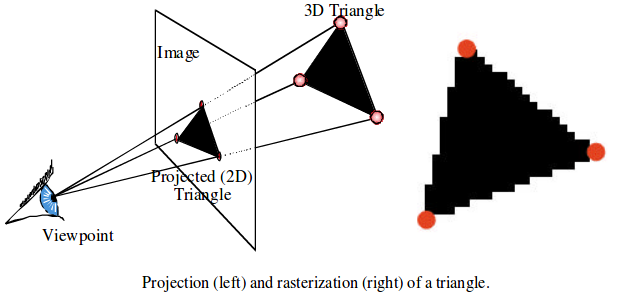
\includegraphics[scale=0.75]{./images/raster.png}
}
\end{figure}

For  richer  rendering,  the  color  of  each rasterized pixel must take into account the optical properties of the object, as we will discuss below. 

\subsubsection{Visibility}

If the scene contains more than one object, occlusions may occur. That is, some objects may be hidden by others. Only visible objects should be represented. Visibility techniques deal with this issue. One classical algorithm that solves the visibility problem is the so-called painter’s algorithm.

It consists in  sorting  the  objects  or  polygons  from  back  to  front  and  rasterizing  them  in  this  order.  This  way,  front-most polygons cover the more distant polygons that they hide. 

\begin{figure}[H]
\centering
\makebox[\textwidth][c]{
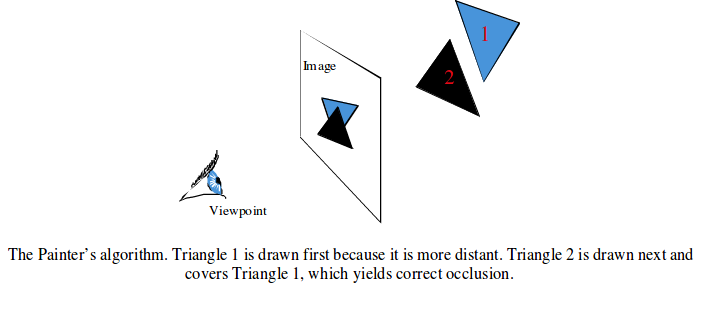
\includegraphics[scale=0.75]{./images/painter.png}
}
\end{figure}

The \textbf{ray-tracing} algorithm does not use a rasterization phase. It sends one ray from the eye and through each pixel of the image. The intersection between this ray and the objects of the scene is computed, and only the closest intersection is considered.

\begin{figure}[H]
\centering
\makebox[\textwidth][c]{
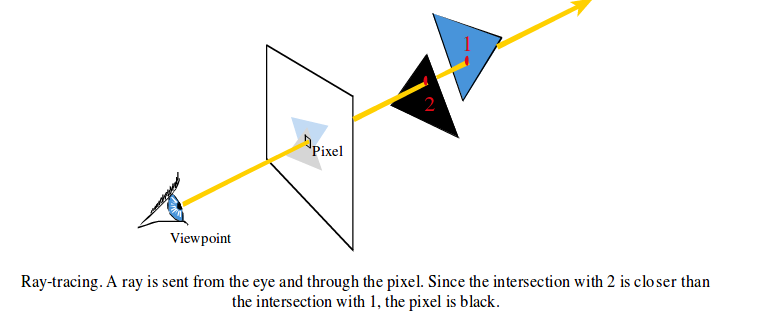
\includegraphics[scale=0.75]{./images/raytrace.png}
}
\end{figure}

The z-buffer method is the most common nowadays (e.g. for computer graphics cards). It stores the depth (z) of each pixel. When a new polygon is rasterized, for each pixel, the algorithm compares the depth of the current polygon and the depth of the pixel. If the new polygon has a closer depth, the color and depth of the pixel  are  updated.  Otherwise,  it  means  that  for  this  pixel,  a  formerly  drawn  polygon  hides  the  current polygon.

\subsubsection{Shading and materials}

Augmenting  the  scene  with  light  sources  allows  for  better  rendering.  The  objects  can  be  
shaded according to their interaction with light. Various shading models have been proposed in the literature. They describe how light is reflected by object, depending on the relative orientation of the surface, light source and viewpoint.

Texture  mapping uses  2D  images  that  are  mapped  on  the  3D  models  to  improve  their  appearance.

Shading and material models only take into account the local interaction of surfaces and light. They do 
not simulate shadows that  are  harder  to  handle  because  they  imply  long-range interactions. A shadow is caused by the occlusion of light by one object. Ray-tracing,  for  example,  can  handle  shadows,  but  requires  a  shadow  computation  for  each  pixel  and  each  light  source.  A  shadow ray is sent from the visible point to the light source. If the ray intersects an object, then the visible point is in shadow.

\begin{figure}[H]
\centering
\makebox[\textwidth][c]{
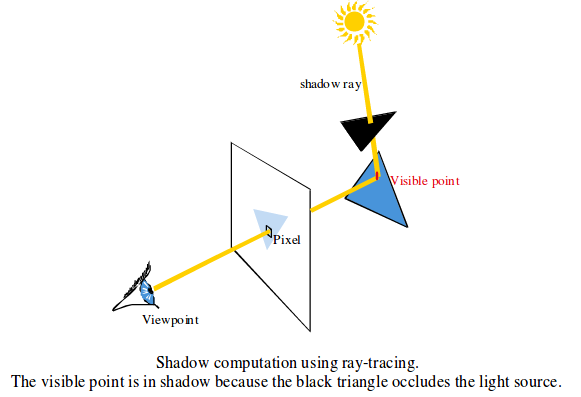
\includegraphics[scale=0.75]{./images/shadow.png}
}
\end{figure}  

More complex lighting interactions can then be simulated. In particular, objects that are illuminated by a 
primary light  source  reflect  light  and  produce indirect  lighting.  This  is  particularly  important  for  indoor scenes. Global lighting methods take into account all light inter-reflections within the scene.

Rendering can be classified in three categories:

\begin{itemize}
\item Non-photorealistic: rendering of scenes in an artistic style, intended to look like a painting or drawing.
\item Photorealistic: rendering of scenes intended to look like indistinguishable from a photo.
\item Physically based: rendering in a way that more accurately models the flow of light in the real world. 
\end{itemize}

See: \url{http://people.csail.mit.edu/fredo/Depiction/1_Introduction/reviewGraphics.pdf}

\subsection{Exercises}

\begin{exercise}
What of the following matrices corresponds to the 2D transformation: translation of an homogeneous vector $(-1,1,1)$ followed by a rotation of angle $\theta = 270^{o}$.
\end{exercise}
\begin{itemize}
\item We have to multiply matrices $((0,-1,0),(1,0,0),(0,0,1))$ and $((0,-1,1),(1,0,2),(0,0,1))$.
\item The answer is $((0,-1,1),(1,0,2),(0,0,1))$.
\end{itemize}


\begin{exercise}
What of the following equivalences between points in homogeneous coordinates are true?
\end{exercise}
\begin{itemize}
\item $(-1,-1,-1) \sim (1,1,1)$ true, take $\lambda = -1$.
\item $(-1,1,1) \sim (1,-1,1)$ false, no $\lambda$ possible.
\item $(-2,2,-1) \sim (1,-1,1)$ false, no $\lambda$ possible.
\item $(-1,1,0) \sim (1,-1,0)$ true, take $\lambda = -1$.
\end{itemize}





\section{Vision humaine}
\subsection{Structure de l'oeil}

Ce cours \'etudie donc la bouce de traitement des images qui part de l'\'ecran, est analys\'ee par l'oeil et le cerveau et g\'en\`ere des actions qui sont per\c{c}ues par l'ordinateur. Nous nous concentrons ici sur la \textbf{perception visuelle}.

Le point essentiel de ce cours est de montrer \textbf{qu'une grande partie de la perception visuelle se passe dans le cerveau}. C'est le cas de la construction des couleurs, comme nous le verrons plus loin, mais aussi de certaines illussions visuelles, comme la perception du triangle de Nakizsa: les bords du triangle ne sont pas dans l'image mais construits par le cerveau.

\begin{figure}[H]
\centering
\makebox[\textwidth][c]{
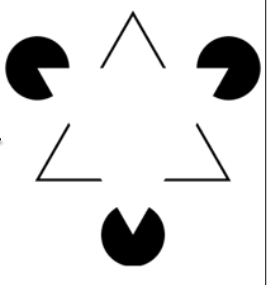
\includegraphics[scale=0.55]{./images/triangle.png}
}
\caption{Triangle de Nakizsa}
\end{figure}

Voici la structure d'un oeil dont 4 \'el\'ements sont particuli\`erement pertinents pour le cours Visual Computing.

\begin{figure}[H]
\centering
\makebox[\textwidth][c]{
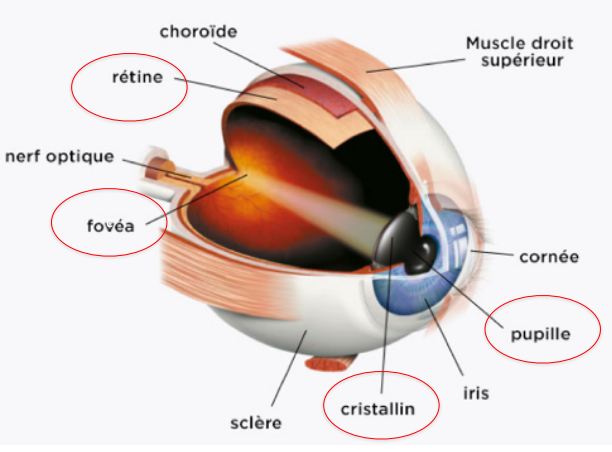
\includegraphics[scale=0.55]{./images/oeil.png}
}
\end{figure}

\begin{itemize}
\item \textbf{pupille}: contr\^ole la quantit\'e de lumi\`ere qui entre dans l'oeil. Sa taille est contr\^ol\'ee par des mouvements des muscles de l'iris qui agissent par r\'eflexe \`a la quantit\'e de lumi\`ere. 
\item \textbf{cristallin}: c'est une lentille bi-convexe qui concentre plus ou moins les rayons lumineux sur la r\'etine. il permet de garder une image nette \`a des profondeurs de champs diff\'erents. Les muscles autour du cristallin l'\'etirent lorsque l'objet regard\'e s'\'eloigne, un ph\'enomene appel\'e \textbf{accomodation}.
\item \textbf{r\'etine}: sorte d'\'ecran plac\'e au fond de l'oeil. Elle est la partie de l'oeil qui capte les photons gr\^ace a un grand nombre de photorecepteurs. Elle couvre le 75 \% de la surface interne de l'oeil.
\item \textbf{macula et fov\'ea}: la macula est la partie centrale de la r\'etine situ\'ee dans l'axe de la r\'etine.  La fov\'ea est une partie de la macula, une p\'etite d\'epression qui correspond \`a la zone qui nous donne la plus grande activit\'e visuelle. Elle comprend une tr\`es forte densit\'e de certains photor\'ecepteurs appel\'ees \textbf{c\^ones} alors que le reste de la macula comporte d'avantage des r\'ecepteurs appel\'es \textbf{b\^atonnets}.
\end{itemize}

Les b\^atonnets et les c\^ones sont des cellules photosensibles. Les b\^atonnets ne per\c{c}oivent pas les couleurs mais sont plus sensibles aux \textbf{niveaux de gris}. Ils permettent notamment la vision par faible luminosit\'e. Ils semblent aussi impliqu\'es dans la \textbf{vision p\'eriph\'erique} pour la perception du mouvement. Environ la r\'etine contient 100 millions.

Les c\^ones se situent dans la fov\'ea. Ils sont environ 6 millions. Ils ont besoin d'avantage de lumi\`ere et sont responsables de la perception de la couleur. En r\'ealit\'e, les c\^ones ne reconnaissent pas la couleur mais nous poss\'edons 3 types de c\^ones sensibles \`a des longueurs d'onde diff\`erentes. Les c\^ones n'envoient pas un message de couleur au cerveau mais lui communiquent le nombre des photons quie les ont heurt\'es. Le \textbf{daltonisme} r\'esulte du fait que certains types de c\^ones ne poss\`edent pas les pigments photosensibles qui captent les photons.

Il existe cependant, dans chaque oeil, une zone d\'epourvue de r\'ecepteurs car c'est le point d'ancrage du nerf optique qui conduit les informations au cerveau. Il s'appelle le \textbf{point aveugle}: tout objet situ\'e dans l'axe r\'etine-point aveugle sera invisible pour cet oeil. Si nous avos les deux yeux ouvert, l'objet sera toujours visible par un oeil. 

En classe, nous font l'exper\'erience suivante. Fermez l'oeil droit. Regardez le losange rouge avec l'oeil gauche. Le professeur traverse l'\'ecran doucement. Vous percevez le professeur en vision p\'eriph\`erique mais il va dispara\^itre un moment.

La structure de la r\'etine d\'efinit notre acurit\'e visuelle dans les diff\'erent zones de notre champ de vision. Notre vision la plus pr\'ecise se limite \`a un angle de 5 degr\'es. N\'eanmoins notre oeil est sensible aux mouvements p\'eriph\'eriques. Il ne glisse pas de mani\`ere continue sur le texte mais l'explore par saccades (voir eye tracking). L'oeil se pose pendant des courtes pauses ou \textbf{fixations} d'un quart de second. Puis, il se d\'eplace tr\`es rapidement vers un autre endroit, ce qu'on appelle une \textbf{saccade}. L'oeil pr\'el\`eve de l'information quand il fait une fixation alors qu'il est aveugle pendant la saccade.

\begin{figure}[H]
\centering
\makebox[\textwidth][c]{
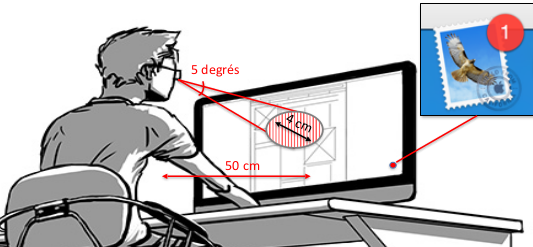
\includegraphics[scale=0.55]{./images/fixation.png}
}
\end{figure}

Quelle quantit\'e d'information visuelle est-elle comprise dans cette zone fov\'eale de 4 cm de diam\`etre?. Cela d\'epend de 6 param\`etres \'enum\`er\'es \`a continuation:

\begin{itemize}
\item l'acurit\'e visuelle de l'utilisateur, de sa distance,de ses lunettes !
\item zoom choisi par l'utilisateur ! 
\item Propri\'et\'es de l'\'ecran:
\begin{itemize}
\item dimensions: longueur de la diagonale (par exemple 13 pouces).
\item d\'efinition: nombre de pixels.
\item r\'esolution: nombre de pixels par pouce carré.
\item profondeur: nombre de bits utilis\'e par chaque pixel.
\end{itemize}

Le	nombre	de	pixels	par	\'ecran	n'a	pas	cess\'e	d’augmenter....
\end{itemize}

Les 3 types de c\^ones envoient chacun un nombre de stimulations \'electriques en fonction du nombre de photons qui les ont heurt\'e. C'est donc le cerveau humain, notamment le \textbf{cortex visuel}, qui int\`egre ces 3 informations pour d\'eterminer la couleur. 

Il semblerait que notre cerveau soit capable de distinguer 10 millions de couleurs. attention, il ne s'agit pas de leur donner un nom mais de d\'etecter que deux couleurs sont diff\'erents. Le nombre de 10 millions d\'epend donc du protocole exp\'erimental utilis\'e, ce qui explique qu'il n'y ait pas consensus. Mais cela signifierait qu'un \'ecran qui a une profondeur de pixel de 24 bits peut g\'en\`erer d'avantage des couleurs que ce que l'oeil humain peut discriminer. 

Dans quelques images on peut voir que la m\^eme diff\'erence en pourcentage de cyande est ou non est perceptible. Il s'explique par la faible pr\'ecision du syst\`eme.

La taille d'un fichier image d\'epend donc du nombre des points dans cette image ainsi que du nombre des bits d'information par point, c'est à dire la profondeur du pixel. Heuresement, ce nombre est ensuite diminu\'e par des \textbf{m\'ethodes de compr\'ession d'image}. D'autres cours de l'EPFL traitent abondamment des m\'ethodes de compression. Apr\'es une compression \textbf{"lossless"}, la d\'ecompression du fichier permet de retrouver exactement chaque bit d'information du fichier original. C'est le cas de fichiers .ZIP. Dans une m\'ethode \textbf{"lossy"}, ce n'est pas le cas. Par example, si on prend la moyenne de couleur entre pixels voisins, un pixel blanc et un noir deviendront deux pixels gris apr\'es la d\'ecompression on pourra d\'eterminer s'ils s'agissait au d\'epart de deux gris ou d'un blanc et d'un noir. La question est de savoir combien d'information peut \^etre perdu \`a la d\'ecompression sans que l'oeil humain ne s'en aper\c{c}oive. En ce qui concerne les images, les standards \textbf{PNG} et \textbf{GIF} sont "lossless" alors que \textbf{JPEG} est "lossy".

\subsection{L'effet Stroop}

Les transparents qui pr\'ec\`edent concernaient la capacit\'e de distinguer deux couleurs. Il ne s'agisait pas de les nommer, ce qui est une t\^ache cognitive (retrouver le nom dans sa m\'emoire \`a long-terme). Voici une exp\'erience qui montre les interf\'erences entre la perception et la cognition. 

\begin{figure}[H]
\centering
\makebox[\textwidth][c]{

\includegraphics[scale=0.55]{./images/stroop.png}
}
\end{figure}

Stroop a d\'ecouvert un effet int\'eressant li\'e \`a la t\^ache suivante: le sujet doit lire un nom de couleur \'ecrit soit dans la couleur du nom soit dans une autre couleur. Il faut nommer la couleur du mot. L'experience au CHILI est un peu diff\'erente: il faut dire si l'\'enonc\'e est correct. 

Le temps n\'ecessaire pour \'enoncer la couleur d'un mot est plus \'elev\`ee si le mot d\'esigne une autre couleur. Ce ph\'enomene \textbf{d'interf\'erence} r\'esulte du fait qu'on ne puisse s'emp\^echer de lire le mot, de lui donner une \textbf{valeur s\'emantique}. La perception ne se fait de mani\`ere independante des autres activit\'es du cerveau, comme nous allons continuer \`a le d\'emontrer.

Comme illustr\'e au d\'ebut de ce cours, la couleur n'est pas per\c{c}ue par l'oeil mais reconstruite par le cortex visuel en fonction du nombre de signaux re\c{c}us par les trois types de c\^ones. C'est aussi dans le cerveau que se construisent la perception du mouvement, les effets d'amor\c{c}age et la perception de la profondeur.

\subsection{Perception du mouvement}

La perception du mouvement doit forc\'ement r\'esulter de la sucession d'images, celles-ci ne sont pas gard\'ees dans l'oeil mais envoy\'ees instantann\'ement au cerveau. Les avis divergent sur le nombre d'images qu'un oeil peut percevoir par secondes. Il semblerait que la r\'etine puisse capter plus de 100 images par seconde (entre 75 et 150), certains parlent de 1000 fps, le point est controvers\'e. Alors pourquoi le cin\'ema s'est-il fix\'e sur le standard de 24 images par secondes? Parce qu'avec 24 images par secondes, voire \`a partir de 16, nous percevons les mouvements commme \'etant continus. Ce nombre de 24 ne r\'epose pas sur une r\'ealit\'e physiologique mais sur un standard \'etablit aux premi\'eres heures du cin\`ema. Aujourd'hui certaines TV haut r\'esolution proposent 120 images par secondes voire 240 pour les \'ecrans LEDs, on parle m\^eme de TV \`a 480 fps. Le d\'ebat consiste \`a savoir si ces fr\'equences offrent une diff\'erence perceptible de confort visuel.

Pourquoi per\c{c}oit-on des images qui se suivent comme un mouvement continu?

\subsubsection{Hypoth\`ese 1: persistence r\'etinienne}

La premi\`ere hypoth\`ese, aujourd'hui critiqu\'ee par les scientifiques, mais toujours r\'epandue dans l'opinion publique, serait que la r\'etine garde un moment l'information avant que les cellules photor\'eceptrices qui ont \'et\'e excit\'ees par un photon ne retournent \`a leur \'etat de repos.

L'image resterait environ entre 1/12 et 1/25 de seconde "imprim\'ee" dans la r\'etine, donc, d\`es 24 images par seconde, on percevrait une continuit\'e. Le film du cheval ne comporte que 12 images par seconde, on voit que le mouvement n'est pas fluide mais on re\c{c}oit n\'eanmoins le mouvement. L'hypoth\`ese de la persistence r\'etinienne est aujourd'hui abandonn\'ee au profit de l'hypoth\`ese suivante.

\subsubsection{Hypoth\`ese 2: effet phi et effet beta}

L'effet phi est la sensation visuelle de mouvement provoqu\`ee par l'apparition d'images per\c{c}ues successives, susceptibles d'\^etres raccord\`ees par un d\'eplacement ou une transformation. C'est le cerveau qui "comblerait" les images interm\'ediaires, qui imagine le mouvement. L'effet beta est la m\^eme illusion de mouvement cr\'e\'e par des images statiques, alors que l'effet phi repose sur des images qui clignotent.

En r\'esum\'e, les hypoth\`eses qui attribuent la construction de la continuit\'e du mouvement au cerveau dominent aujourd'hui celles qui l'attribuent \`a l'oeil. Ce ph\`enom\`ene qui expliquerait le mouvement apparent dans les "flipbooks" et "thaumatropes".

\subsection{Perception de l'amor\c{c}age}

La perception est typiquement en m\'ecanisme bottom-up: je per\c{c}ois l'image d'un objet et je l'associe aux objets que je connais d\'ej\`a. On parle de processus-bottom up: l'image de l'objet s'imprime sur la r\'etine qui transmet au cortex visuel lequel communique avec les autres composantes du syst\`eme cognitif.

Ce texte illustre le processus \textbf{bottom-up}:

Le fait qu'un \'el\'ement visuel brise la r\'egularit\'e du texte. Rome \'etant \'ecrit en rouge, permet de le s\'electionner plus rapidement. 
Le fait que Rotterdam se mette \`a trembler attire notre attention.
Le fait que Moscu se d\`epala attire notre attention.

Parmi l'ensemble des stimuli pr\'esent\'es, certains ont des propri\'et\'es qui attirent notre attention, celui-ci brise une r\`egularit\`e \'etablie par l'ensemble du stimulus.

\begin{figure}[H]
\centering
\makebox[\textwidth][c]{
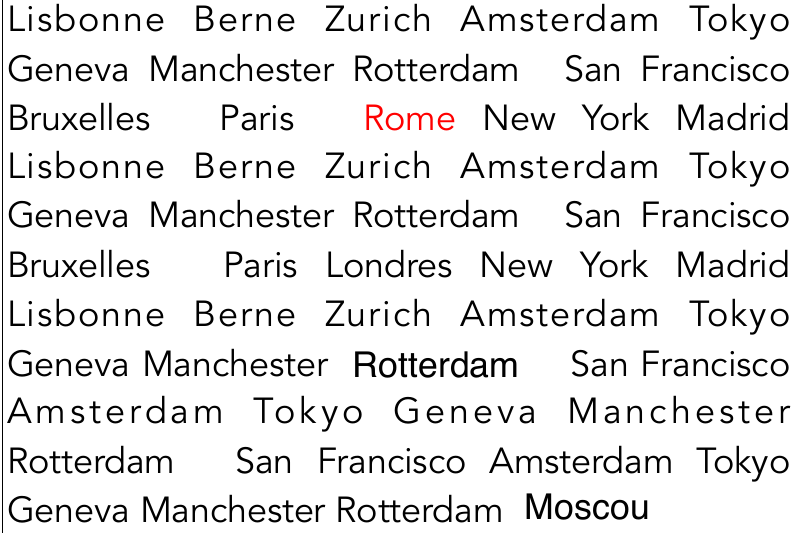
\includegraphics[scale=0.35]{./images/cites.png}
}
\end{figure}

Dans cette image, le taxi en couleur \'eclatante d\'eclenche les processus bottom-up. Notre attention devrait donc surtout s\'electionner le taxi. Mais un autre processus intervient: il n'est pas normal de voir un \'el\'ephant en libert\'e dans les rues d'une ville. Sa pr\'esence entre en conflit avec ce qu'on attend en regardant une image de ville nocturne...Dans ce cas, c'est notre cognition qui dirige notre attention et non pas les propri\'et\'es physiques de l'image qui guident l'attention. On parle dans ce cas de processus \textbf{top-down}. La perception d'objets dans une image est fortement influenc\'ee par nos attentes, nos exp\'eriences, nos connaissances,...La perception d'objets dans une image est fortement influenc\'ee par nos attentes, nos exp\'eriences, nos connaissances,...

\begin{figure}[H]
\centering
\makebox[\textwidth][c]{
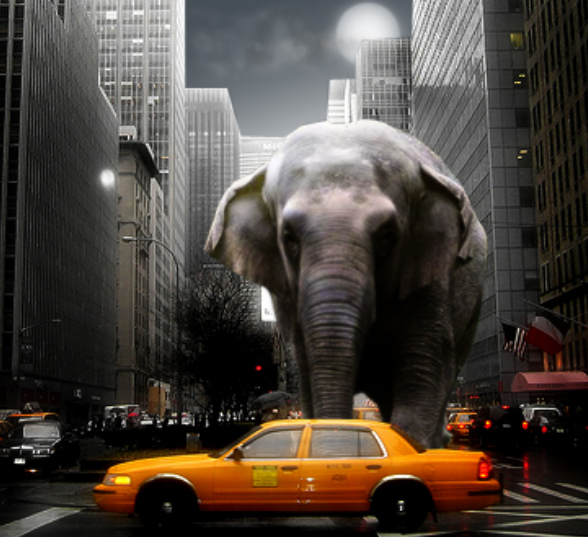
\includegraphics[scale=0.35]{./images/elephant.png}
}
\end{figure}
	
\textbf{L'effet d'amor\c{c}age ou priming effect} consiste \`a pr\'esenter un stimulus (l'amorce) afin d'influencer la perception d'un autre stimules (la cible). L'amorce \'etait les images pr\'ealables de vase ou de profils et la cible \'etait l'image ambigue. Nous percevons beacoup d'objets mais les processus bottom-up guident notre attention sur certains objets particuliers, c'est \textbf{l'attention s\'elective}. Un example bien connu dans la perception auditive est le \textbf{cocktail party effect}: si je parle avec plusieurs personnes au milieu d'une soir\'ee bruyante, je per\c{c}ois n\'eanmoins les conversations externes car, si quelqu'un prononce mon nom une autre table, ceci attirera n\'eanmoins mon attention.

\begin{figure}[H]
\centering
\makebox[\textwidth][c]{
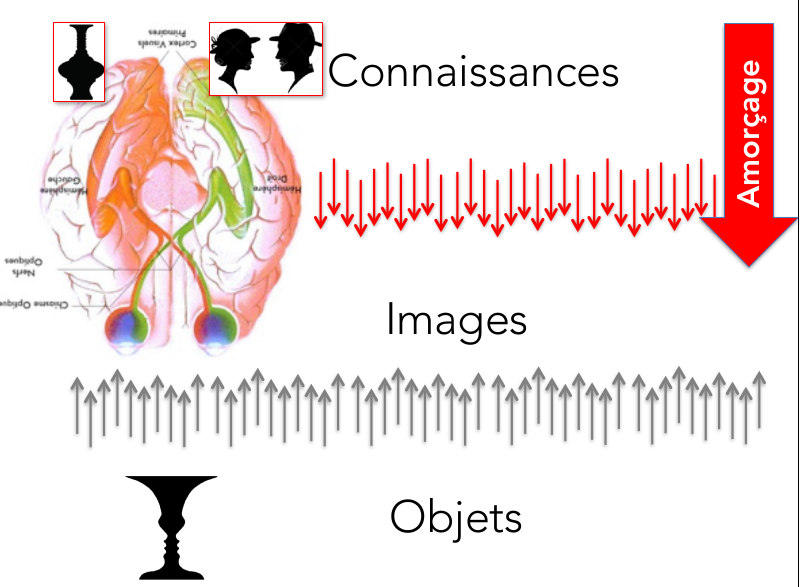
\includegraphics[scale=0.35]{./images/amorce.png}
}
\end{figure}

\subsection{Perception de la profondeur}

La perception de la profondeur est construite par le cerveau qui r\'econcilie les informations provenant des deux yeux. Chaque oeil envoie un demi-champ de vision \`a chaque h\'emisph\`ere. Il utilise des indices diff\'erents:

\subsubsection{Indices binoculaires}

Le principe de base est simple, l'angle de l'image sur la r\'etine d\'etermine la distance d l'objet par triangulation.

\subsubsection{Indices monoculaires}

M\^eme avec un seul oeil ouvert, nous avons une certaine perception de la profondeur gr\^ace \`a diff\'erents indices. 

\textbf{La perspective}: deux lignes parall\`eles qui s'\'eloginent du point de vision sont per\c{c}ues comme se rapprochant. On peut en profiter avec un oeil ferm\'e mais il n\'ecessite un d\'eplacement ce qui n'est pas tr\'es diff\'erent d'un principe binoculaire ou multioculaire.

\textbf{L'effet parralaxe}: c'est un m\'ethode pour obtenir la profondeur en faisant d\'eplacer les objets en premier plan plus rapidement que les objets en deuxi\`eme plan.

\textbf{L'effet kinetic depth}: les mouvements de l'objet donnent une perception de sa structure en 3D.


\begin{figure}[H]
\centering
\makebox[\textwidth][c]{

\includegraphics[scale=0.35]{./images/kinetic.png}
}
\end{figure}

\textbf{L'occlussion}: m\^eme en 2D, cette image donne l'impression que le rectangle jaune se trouve en avant-plan du rectangle bleu. Cet effet peut \^etre retourn\'e, par exemple si la forme bleu n'est pas un rectangle mais un polygone en forme de U couch\'e. Les ombres constintuent un cas particulier d'occlusion.

\begin{figure}[H]
\centering
\makebox[\textwidth][c]{
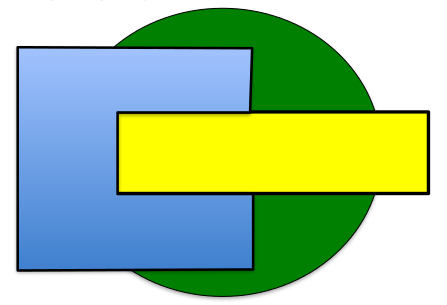
\includegraphics[scale=0.35]{./images/occlusion.png}
}
\end{figure}

\textbf{La taille relative}:

Malgr\'e l'absence de lignes de perspective, les objets plus petits sont per\c{c}us comme plus \'elogin\'es, sauf si la s\'emantique de l'image nous fournit une autre interpr\'etation de la diff\'erence de taille. Sans indices externes, on ne peut estimer la distance d'un objet dont on ne conna\^it pas la taille. 

\textbf{Position par rapport \`a l'horizon}:

Le fait de briser la ligne d'horizon est une propri\'et\'e des objets \'eloign\'es.

\subsection{Recr\'eer la profondeur en 2D}

La diff\'erence de nettet\'e de l'image entre l'avant plan et l'arri\`ere plan fournit une perception de la profondeur. 

\textbf{Finesse de la texture}: la profondeur est communiqu\'ee en augmentant la finesse des textures en avant plan et en la r\'eduisant dans le fond.

\textbf{Brouillard de distance}: un effet brouillard est utilis\'ee dans les jeux pour donner une perception de la profondeur. Il permet aussi de ne pas calculer les d\'ecors tr\`es \'eloign\'es.

\subsection{Remarques}

Chaque h\'emisph\`ere traite une demi-image et la partage avec l'autre h\'emisph\`ere. Mais que se passe-t-il si l'information ne passe plus entre les deux h\'emisph\`eres? Ceci arrive notamment dans des cas graves d'\'epilepsie qui conduit \`a une intervention chirugical qui sectionne le corps calleux, le faisceau d'axones qui connecte les deux h\'emisph\`eres.

\begin{figure}[H]
\centering
\makebox[\textwidth][c]{
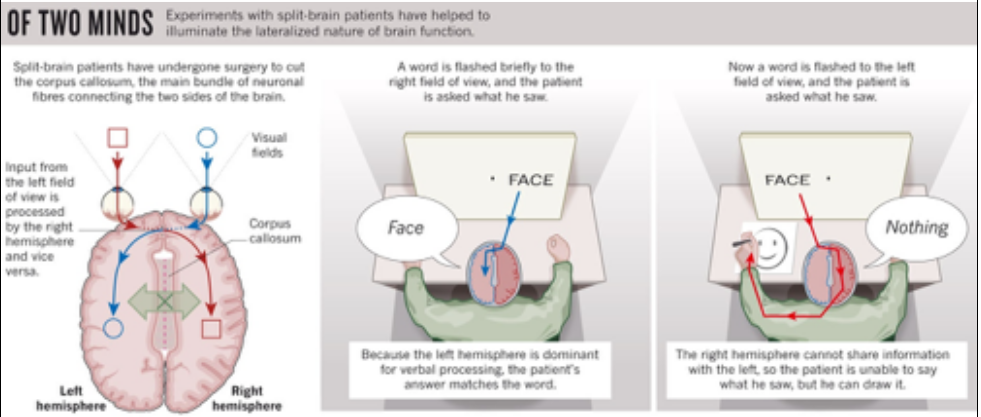
\includegraphics[scale=0.35]{./images/splitbrain.png}
}
\end{figure}

\textbf{Exp\'erience du Split Brain}: gr\^ace \`a un dispositif technique, on projectte par exemple deux demi-images droites qui ne sont envoy\'ees qu'\`a l'hemisph\`ere gauche. Celui-ci \'etant sp\'ecialis\'e dans le traitement du langage, le sujet peut dire "face". Si ces deux demi-images sont transmises \`a l'h\'emisph\`ere droit, le sujet ne pourra pas lire le mot mais pourra dessiner l'objet.

\textbf{Stimuli subliminaux} (hypoth\`ese controvers\'ee):
\begin{itemize}
\item Si un stimulus visuel est inf\'erieur au seuil de perception (en taille, dur\'ee, longueur d'ondes), il serait n\'eanmoins per\c{c}u par notre inconscient.
\item Il aurait de ce fait une influence non-contr\^olable sur notre comportement.
\end{itemize}

\subsection{Exercises}

\begin{exercise}
Quelles composantes de l'oeil lui permettent de r\'ealiser les performances suivantes?
\end{exercise}
\begin{itemize}
\item Lire des petits caract\'eres \`a l'\'ecran. (cristallin)
\item Discriminer un mot en bleu d'un mot en rouge. (c\^ones)
\item S'adapter \`a la distance de l\'ecran pour obtenir une image nette. (cristallin)
\item Lisant du texte en haut de l'\'ecran, d\'etecter que l'ic\^one mail se met \`a clignoter en bas d'\'ecran (b\^atonnets)
\item Lors d'une promenade nocturne, reconna\^itre des objets dans la p\'enombre (b\^atonnets)
\end{itemize}

\begin{exercise}
O\`u se passent les ph\'enom\`enes suivants? 
\end{exercise}
\begin{itemize}
\item L'effet stroop (cerveau)
\item La persistance de l'image (oeil)
\item L'effet phi ou beta (cerveau)
\item L'effet parallaxe (cerveau)
\end{itemize}












\section{Cognition humaine}
Ce chapitre concerne diff\'erents processus r\'eunis sous le terme cognition. Nous avons vu qu'il n'y a pas de distinction stricte entre la perception et la cognition puisque la derni\`ere influence la premi\`ere, mais nous nous int\'eresons ici aux aspects impliqu\'es dans la r\'esolution de probl\`emes. Nous nous int\'eressons aux fonctions que ces m\'emoires offrent \`a l'utilisateur d'un syst\`eme informatique.

La psychologie cognitive est une branche de la psychologie qui s'int\'eresse aux grandes fonctions de notre intellect. Nous nous int\'eresserons en particulier dans la m\'emoire, raisonnement, connaissances et apprentissage. D'autres aspects sont aussi important dans l'interaction personne-computer mais on va se concentrer sur les concepts fondamentaux. 

La psychologie cognitive porte un \textbf{regard fonctionnel} sur la m\'emoire. Elle d\'efinit trois types de m\'emoire qui correspondent \`a des fonctions cognitives distinctes:

\begin{itemize}
\item M\'emoire sensorielle: retient les \'even\'ements pass\'ess dans le dernier secondes.
\item M\'emoire de travail ou m\'emoire \`a court terme: retient les \'even\'ements pass\'ess dans les derniers dix minutes.
\item M\'emoire \`a long terme: retient les \'even\'ements pass\'ess \`a long terme. 
\end{itemize}

Le lien entre la fonction cognitive et le substrat biologique du cerveau est l'objet des \textbf{neurosciences}. Les trois m\'emoires d\'ecrites fonctionnellement (par performances ou oublis des sujets) ont \'et\'e mises en relation avec l'activation de zones distinctes du cerveau.Ces trois m\'emoires sont souvent pr\'esent\'ees comme des bo\^ites ou des tiroirs dans la grande armoire. C'est une simplification grossi\`ere. Une hypoth\`ese est par exemple que m\`emoire \`a court terme serait simplement un sous-ensemble de la m\'emoire \`a long terme qui a \'et\'e pr\'e-activ\'e. 

La mani\`ere la plus simple de comprendre notre cognition est d'analyser pourquoi nous commettons des erreurs.  On peut faire \c{c}a en mesurant la charge cognitive. Exemple: genealogy game. 

Normalement, la capacit\'e de notre m\'emoire de travail est limit\'ee entre cinq et neuf \'el\'ements. Pour la mesurer on peut utiliser:

\begin{itemize}
\item Mesures physiologiques: EEG, fr\'equence cardiaque, mouvement oculaires, contractions musculaires.
\item Mesures subjectives: par questionnaire apr\`es la t\^ache.
\item Mesures de performance: la "dual task".
\end{itemize}

La t\^ache 1 est de difficult\'e constante alors qu'on augmente progressivement la difficult\'e de la t\^ache 2. \`A un certain seuil de difficult\'e, la difficult\'e de la t\^ache 2 va conduire \`a une augmentation du nombre d'erreurs sur la t\^ache 1, bien que celle-ci n'ait pas augment\'e en difficult\'e. Cette interf\'erence d'une t\^ache sur l'autre t\'emoigne d'une surcharge cognitive.

\begin{figure}[H]
\centering
\makebox[\textwidth][c]{
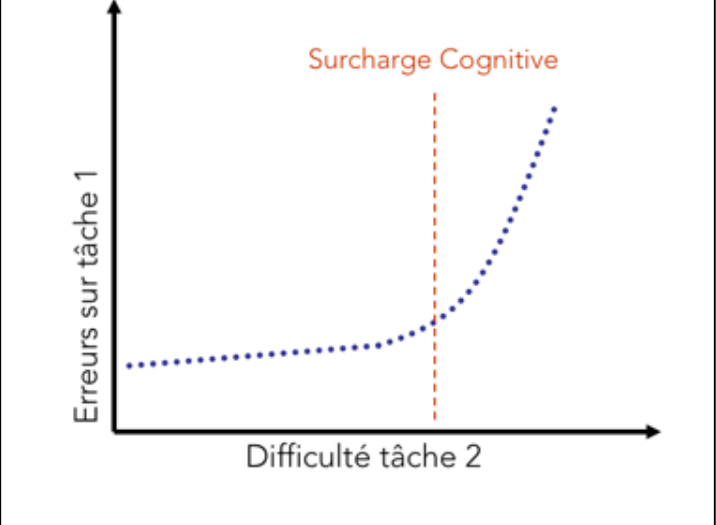
\includegraphics[scale=0.35]{./images/dual.png}
}
\end{figure}

Est-il vraiment possible que nous puissions r\'esoudre des t\^aches complexes, telles que la programmation, avec une m\'emoire de travail qui serait limit\'ee \`a sept slots? Lorsqu'on programme, on est totalement concentr\'e afin de maintenir en m\'emoire le nom des variables, des fonctions ou des classes utilis\'ees, leur position dans le code, les sous-fen\^etres, etc. 

\begin{figure}[H]
\centering
\makebox[\textwidth][c]{
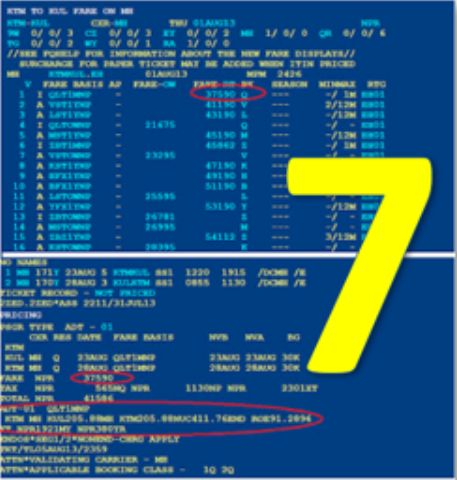
\includegraphics[scale=0.35]{./images/prof.png}
}
\end{figure}

Ce type d'interface est utilis\'ee par les professionnels pour r\'eserver des billets d'avion. \`A la diff\'erence de l'interface web que nous utilisons pour r\'eserver un vol cette interface contient une quantit\'e \'enorme d'information. Comment les utilisateurs peuvent-ils g\'erer cette quantit\'e alors qu'ils ont les m\^emes limites que tout le monde en termes de charge cognitive? Un utilisateur expert lit en fait cet \'ecran non comme 545 \'el\'elements mais comme un nombre limit\'e de blocs d'information.

De la m\^eme mani\`ere un conducteur expert parvient \`a mener un grand nombre d'op\'erations en parall\`ele. Lorsqu'on apprend \`a conduire, changer de vitesse repr\'esente plusieurs op\'erations cognitives distinctes. Plus tard, ce jeu d'op\'erations ayant \'et\'e automatis\'e ou "compil\'e", il ne mobilise plus qu'une partie mineur de notre m\'emoire de travail. Les interfaces proposent aussi des moyes de compilation. Il existe de nombreuses \'etudes qui diff\'erencient novices et experts. La compilation des connaissances est l'un des \'el\'ements, mais ce n'est pas le seul.

\subsection{Split attention effect}

L'effet de "split attention" d\'ecrit l'augmentation de la charge cognitive qu'implique les aller-retours visuels entre une figure et sa l\'egende, ou, de mani\`ere plus g\'en\'erale, entre deux sources d'information. Combien d'informations par \'ecran est-il optimal de pr\'esenter dans un seul \'ecran? Minimiser les information par \'ecran n'est pas la solution car la plupart des t\^aches demandent de mettre en relation plusieurs \'el\'ements d'information. D\'ecomposer l'information en n \'ecrans n'est pas id\'eal puisque cela aboutit \`a la morceler. Le fait de structurer l'information r\'eduit la charge cognitive. 

\begin{figure}[H]
\centering
\makebox[\textwidth][c]{
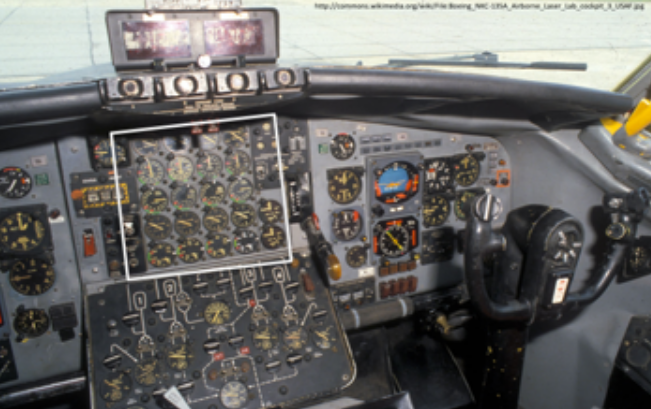
\includegraphics[scale=0.35]{./images/structure.png}
}
\end{figure}

Par exemple, si n cadrans ont des aiguilles qui devraient \^etre parall\`eles, le contr\^ole de ces n \'ecrans ne n\'ecessite pas de lire les indications de chaque cadran car il suffit de contr\^oles le parall\'elisme.


On peut calculer la charge cognitive avec la fomule suivante:

$$\text{Charge cognitive} = \frac{\text{Quantit\'e d'information}}{\text{Niveau d'expertise} \cdot \text{Qualit\'e du design}}$$

Ici le design de l'interface est la seule variable sur laquelle nous avons de l'influence. 

\subsection{Distributed cognition}

Distributed cognition is an approach to cognitive science research that deploys models of the extended mind by taking as the fundamental unit of analysis "a collection of individuals and artefacts and their relations to each other in a particular work practice".

Par exemple un programmeur utilise l'\'ecran pour \'etendre sa m\'emoire de travail car elle pr\'esent l'ensemble des informations n\'ecessaires \`a r\'ealiser son travail. Une personne aveugle utilise sa canne pour explorer l'espace. L'id\'ee c'est d'\'etudier le syst\`eme cognitif dans son ensemble, compos\'e d'un ou plusieurs cerveaux et de leurs outils.

Dans la m\'emoire \`a long terme, on distingue deux formes de connaissances: connaissances d\'eclaratives et connaissances proc\'edurales. Les connaissances d\'eclaratives comprennent les concepts, id\'ees, principes, faits ou th\'eories. Les connaissances proc\'edurales d\'ecrivent les mani\`eres d'op\'erer, faire, d\'ecomposer ou calculer. Il y a une r\'ealimentation entre les deux. 

Dans l'ensemble des connaissances d\'eclaratives on distingue la m\'emoire s\'emantique et la m\'emoire \'episodique. La m\'emoire s\'emantique retient les faits, concepts ou d\'efinitions. La m\'emoire \'episodique retient les ev\'enements pass\'es ou imagin\'es. 

\begin{figure}[H]
\centering
\makebox[\textwidth][c]{
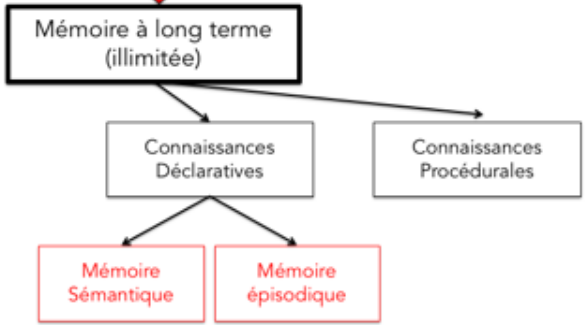
\includegraphics[scale=0.35]{./images/semantique.png}
}
\end{figure}

A \textbf{mental model} is an explanation of someone's thought process about how something works in the real world.

La m\'emoire s\'emantique aide \`a construire les mod\`eles mentaux. Ce mod\`eles evoluent avec l'exp\'erience et sont souvent li\'es au contexte dans lequel ils ont \'et\'e acquis. Ils ne sont pas forc\'ement corrects, ni complets et ils peuvent comprendre des contradictions. Il s'agit des explications simplifi\'ees des ph\'enom\`enes complexes et contiennent une estimation de leur validit\'e qui permet de les utiliser malgr\'e leur incertitude. Ils aident \`a comprendre certaines erreurs des utilisateurs.

\subsection{Metacognition}

La metacognition d\'esigne la connaissance des connaissances ("je ne suis pas bon pour m\'emoriser les noms", "je suis pr\^et pour l'examen", "pour des probl\`emes de ce type, je pr\'ef\`ere faire un sch\'ema") et le raisonnement sur le raisonment ("je devrais repartir d'un \'etape pr\'ec\'edente" ou quelle est la meilleure m\'ethode pour ce probl\`eme?).

\begin{figure}[H]
\centering
\makebox[\textwidth][c]{
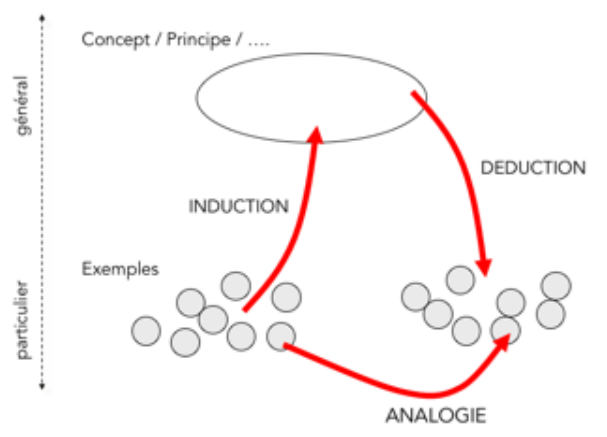
\includegraphics[scale=0.35]{./images/principes.png}
}
\end{figure}


\subsection{Exercises}

\begin{figure}[H]
\centering
\makebox[\textwidth][c]{
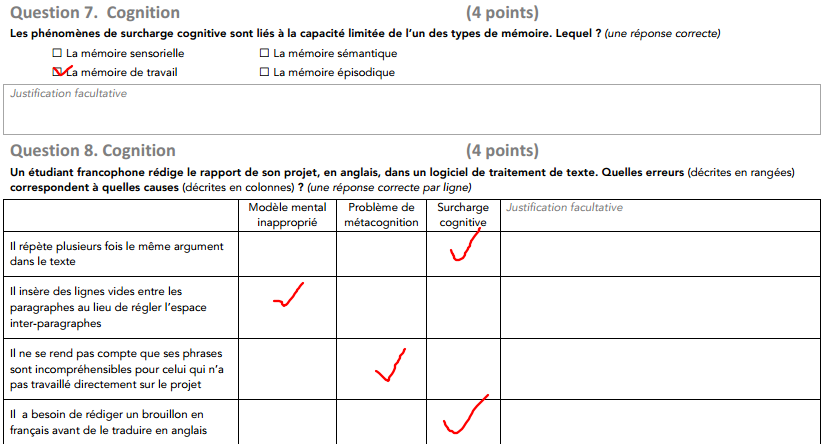
\includegraphics[scale=0.55]{./images/exercise3.png}
}
\end{figure}

























\section{Visualisation de l'information}
Il s'agit maintenant de d\'ecouvrir qu'est-ce qu'il y a dans mes donn\'ees. Comment montrer des choses apart de ce qui est gard\'e dans mon fichier. Par exemple dans le project de ce cours on montre le score obtenu. La visualisation des donn\'ees est tr\`es importante dans le monde de l'informatique d\'ecisionnelle (business intelligence) qui vise \`a donner les moyens pour collecter, consolider, mod\'eliser et restituer les donn\'ees d'une entreprise en vue d'offrir une aide \`a la d\'ecisiion et de permettre au d\'ecideur d'avoir une vue d'ensemble de l'activit\'e trait\'ee.

\subsection{Grammaire visuelles}

Ici on fait la visualisation en trois \'etapes:

1. \textbf{Placer les donn\'ees sur une image de base} de telle sorte que les propri\'t\'es visuelles de l'image refl\`etent les propri\'t'es abstraites des donn\'ees en particulier les relations entre donn\'ees. 

2. Cr\'eer une \textbf{grammaire visuelle} qui met en correspondance les variables des donn\'ees et les composantes graphiques. Si n\'ecessaire on cr\'ee une grammaire pour chaque dimension.

3. Mettre en \textbf{correspondance} un espace de n dimensions vers un espace de moindre dimensions par des m\'ethodes graphiques et des m\'ethodes statistiques.

\subsection{Principes de conception (Tufte)}

1. Choisir des unit\'es qui conservent du sens \`a travers les comparaisons. Exemple: wage minutes to by a hamburger in each country.

2. Choisir des unit\'es qui ont du sens pour le lecteur. Exemple: gross domestic product (GPD).

3. Choisir des intervalles pertinents. Exemple: a representation with big intervals can lead to not considering the whole information represented.

4. Evaluer les effets du choix des intervalles.

5. V\'erifier \textbf{l'int\'egrit\'e graphique}. Est-ce que l'importance visuelle correspond \`a la quantit\'e repr\'esent\'ee? Ici la perspective ou la r\'epresentation en 3D peuvent entra\^iner un pi\`ege.

6. Minimiser le "chart junk". Eviter les \'el\'ements qui n'apportent pas d'information et risquent de bruiter le message.

7. Optimiser le \textbf{"data ink ratio"}. Le data ink ratio c'est le quotient entre la quantit\'e de "ink" utilis\'ee to montrer le data entre la quantit\'e de "ink" utilis\'ee pour montrer le graphique. Elle devrait \^etre une magnitude \'elev\'ee outre on risque de utiliser trop d'\'elements graphiques pour r\'epresenter le data. Un donn\'ee peut s'identifier parce que si on l'efface, on perd de l'information.

8. Utiliser les \textbf{"small multiple"}. Il s'agit d'une s\'erie de graphiques similaires qui utilisent la m\^eme \'echelle et axes et qui permettent de les comparer facilement.

9. Montrer les co-variations. On montre sur un m\^eme graphique les variations des magnitudes r\'elationn\`ees . Ce qui permet \`a l'oeil de cr\'eer la correlation.

10. Montrer le contexte. Contextualiser l'information pour pr\'eciser son contenu.

\subsection{Distorsions g\'eom\'etriques}

Il n'existe pas de visualisation objective. Visualiser c'est communiquer.

On rencontre fr\'equentement des distorsions des visualizations qui peuvent \^etre forc\'ees ou n\'ecessaires.  

Exemples des \textbf{distorsions forc\'ees}: la repr\'esentation du globe terrestre sur le plan d'une carte. La Winker triple projection essaye de minimiser les distortion en termes de distance, angles et surfaces. La repr\'esentation d'une pyramide sur un plan, par exemple la r\'epresentation d'une montagne comme les Diablerets.

Il y a des autres distortions g\'eom\'etriques qui peuvent \^etre n\'ecessaires pour bien r\'epresenter l'objet sous \'etude. Par exemple le diagramme des lignes de m\'etro doit int\'egrer diff\'erent zones avec \textbf{diff\'erentes densit\'es}. Pour bien faire cette distorsion on peut utiliser des outils comme des \'echelles non-lin\'eaires, l'effet loupe ou des modes interactifs. 

On peut rencontrer des occassions ou il faut "tricher" pour rendre visible ce qui n'est pas visible. Par exemple si on repr\'sente les salaires et les ages d'un groupe des personnes et on veut savoir combien des personnes nous sommes en train d'\'etudier on peut ajouter du \textbf{bruit al\'eatoire ou "jitter"} aux donn\'ees pour rendre tous les points visible. En faisant \c{c}a, la visualization est fausse par respect \`a un axe mais plus correcte par rapport \`a la nature des donn\'es.

Une autre distortion n\'ecessaire peut \^etre \textbf{l'utilization des \'echelles incompatibles}. Par exemple si on veut representer une ascension alpiniste il est important de remarque l'ascension vertical m\^eme s'il est n\'egligeable en comparaison avec l'\'echelle horizontal. Ainsi on fait une exag\'eration dans certaines magnitudes. Une mesure pour d\'eterminer le degr\'e de distortion est le \textbf{Lie factor}. Il est le quotient entre l'effet montr\'e dans le graphique et l'effect montr\'e dans le data. 

Quelques distortions peuvent \textbf{communiquer des id\'ees}. Une carte standard peut \^etre distortion\'e pour montrer des informations sur la population ou le PIB de chaque pays. Le nombre des inscrits dans les cours de l'EPFL peut \^etre represent\'e par pays selon le nombre d'inscrits ou en r\'elation avec le nombre d'utilisateurs d'Internet.

\subsection{Erreurs fr\'equents dans la conception ou interpr\'etation des visualisations}

\begin{itemize}
\item Les couleurs ne fournissent pas d'information.
\item \textbf{L'empilement des graphiques} n\'ecessite de calculer mentalement les comparaisons.
\item Les \textbf{valeurs extr\^emes} \'ecrasent l’information. Une solution est l'utilisation d'\'echelles non-lin\'eaires par exemple l'\'echelle logarithmique.
\item Le syst\'eme g\'en\`ere automatiquement une \'echelle inappropri\'ee qui emp\^eche de faire des comparaisons correctes.
\item \textbf{Ordre des donn\'ees non justifi\'e}. Le pattern visuel produit d\'epend davantage de l’ordre des donn\'ees que des donn\'ees elles-m\^emes.
\item Ordre des donn\'ees innapropri\'e.
\item Les \textbf{points connect\'es} par des traits ne sont pas r\'eellement des donn\'ees li\'ees les unes aux autres.
\item \textbf{Sensibilit\'e de la moyenne aux valeurs extr\^emes}. C'est pour \c{c}a qu'on fait les analyses de variance. Dans les repr\'esentations graphiques de donn\'ees statistiques, la \textbf{bo\^ite \`a moustaches} est un moyen rapide de figurer le profil essentiel d'une s\'erie statistique quantitative.
\item \textbf{Sensibilit\'e des courbes de tendance}.
\item \textbf{Intepr\'eter une corr\'elation comme un lien de causalit\'e}. La corr\'elation peut \^etre en r\'ealit\'e caus\'ee par l'existence d'une \textbf{variable cach\'ee}. Ainsi probablement s'endormir avec une seule chaussure n'est pas la cause de se r\'eveiller avec un mal de t\^ete mais la cause peut \^etre tr\`es bien la consommation d'alcool.
\item Les \textbf{acronymes rares} pour l'utilisateur augmentent sa charge cognitive.
\item Le "split attention effect" augmente la charge cognitive.
\end{itemize}

The \textbf{split-attention effect} is a learning effect inherent within some poorly designed instructional materials. It is apparent when the same modality (e.g. visual) is used for various types of information within the same display. To learn from these materials, learners must split their attention between these materials to understand and use the materials provided.

Les \textbf{visualisations dynamiques} font usage de des utiles particuliers: changement d'\'echelle spatiale (zoom, croll,...), changement d'\'echelle temporelle, changement d'\'echelle des variables, rotations 2D ou 3D, changement de variables, "mouse over" (events that happen when the mouse is over the element)...

\subsection{Exercises}

\begin{figure}[H]
\centering
\makebox[\textwidth][c]{
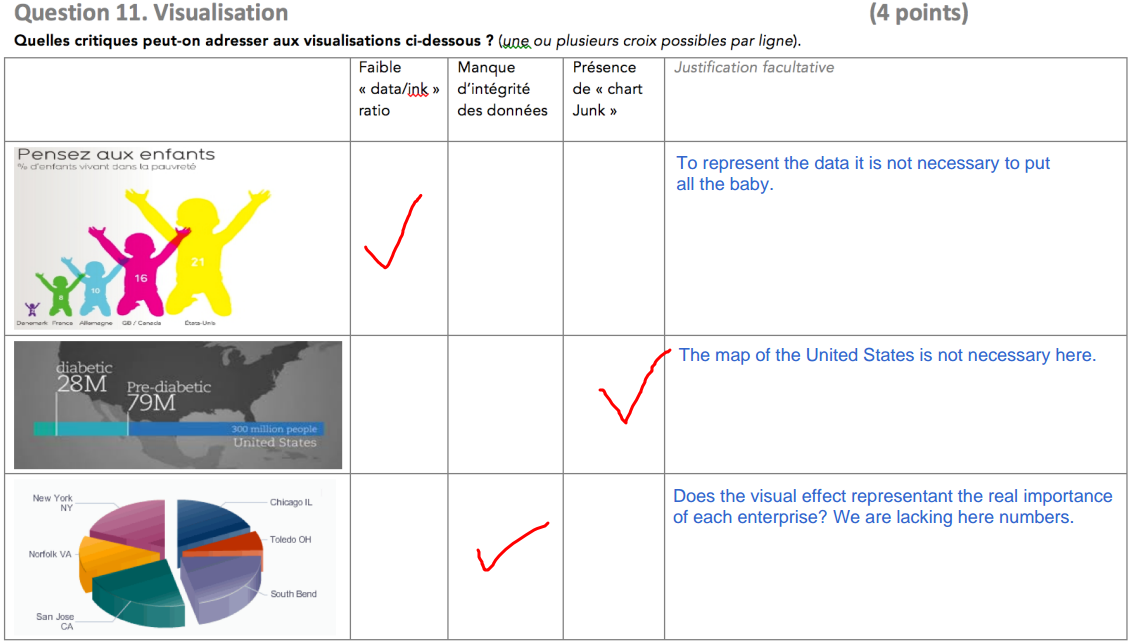
\includegraphics[scale=0.35]{./images/exercise1.png}
}
\end{figure}

\begin{exercise}
En rempla\c{c}ant une visualisation en 3D par un treillis de vues 2D, quels principes de visualisation des donn\'ees sont-ils mis en oeuvre? 
\end{exercise}

Eviter le split attention effet (pas correcte)

Eviter l'occlusion de certaines donn\'ees (correcte)

Eviter le lie factor (pas correcte)

Utiliser les small multiples (correcte)

Utiliser les distorsions (pas correcte)















\section{M\'ecanismes des jeux}
Pour ce chapitre: "The Art of Game Design: A book of Lenses.

Quelle est la diff\'erence entre un jeu et un jouet? Dans un jeu, les buts et les r\`egles sont invent\'es par le concepteur du jeu. Pour un jouet, c'est le joueur qui invente ses propres buts, son histoire, etc. En autres mots, un jeu r\'epond \`a une r\`egle et le jout ne fait place qu'\`a l'imagination.

Dans un jeu, il y a des modalit\'es de jeu diff\'erentes:

\begin{itemize}
\item Free-to-play: les joueurs ont acc\`ess \`a une quantit\'e de contenu importante sans payer. Cependant, cette modalit\'e est normalement bas\'ee dans un model "freemium". Pour acc\`eder \`a toute la fonctionalit\'e il faut payer. 
\item Pay-to-play: un payement est pr\'ecis\'e avant d'utiliser le service la premi\`ere fois.
\item Pay-to-win: dans certes free-to-play jeux, les joueurs peuvent obtenir avantages faces \`a des autres joueurs dans un contexte multiplayer. La critique sugg\`ere de offrir charact\'eristiques additionels sans affecter le "gameplay".
\end{itemize}

Pourquoi un jeu "marche"? Par l'influence des r\'eseaux sociaux, buzz, nouveaut\'e, prix, plateforme, qualit\'es esthetiques si l'on essai. Par des mechanismes qui g\'en\`erent l'engagement, voire l'addiction si on revient. 

\subsection{17 "Game Mechanics"}

On appelle "game mechanics" l'ensemble des m\'ethodes ou r\`egles qui permettent d'interactionner avec le jeu.

\subsubsection{L'espace}

Il ne s'agit pas du graphisme ou du d\'ecor mais l'ensemble des positions qui correspondent \`a un \'etat. Il peut \^etre discret (monopoly, \'echecs) ou continu (billard, war, ski, car) et \^etre uni, bi ou tri dimensionnel. Un exemple de jeu 5-dimensionnel est le jeu des 1000 questions. Ici on peut choisir cinq dimensions ou \'etats pour la difficult\'e, pour le th\'eme ou l'\'etat du joueur. La structure de l'espace peut combiner elements discrets et contius comme dans le Supermario. La structure peut \^etre aussi lin\'eaire, en grille, web ou partition. 

Pour bien comprendre l'espace le joueur doit avoir des bonnes facult\'es de visualisation, de capacit\'e d'orientation. Des tests int\'eressants pour mesurer \c{c}a sont le test du "paper folding" ou la "rotation mentale". Dans le jeu on fournit les outils nec\'essaires pour faciliter la t\^ache: utilisation des cartes ou des rep\`eres.

\subsubsection{Le temps}

Le temps peut \^etre discret (des tours) ou continu (un horloge, un sablier). Si continue il peut \^etre illimit\'e ou limit\'e et inte\'egr\'e dans le score. Le joueur peut parfois l'influencer: ralentir, pauser, acc\'el\'erer ou retourner. 

\subsubsection{Les objets}

Les charcteristiques des objets sont repr\'sent\'es par des constantes ou des variables (ces derni\`eres forment l'\'etat) ainsi comme par un diagramme d'\'etats comme dans le cas du Pacman. Un type pr\'ecis d'objets est form\'e par les personnages et les avatars. Ces personnages peuvent \^etre moins ou plus r\'ealistes. Il existe une hypoth\`ese qselon laquelle plus un robot androide est similaire \`a un \^etre humain, plus ses imperfections nous paraissent monstrueuses. C'est pour cela qu'est utilis\'e le terme de vall\'ee : il s'agit d'une zone \`a franchir dans laquelle chaque progr\`es fait vers l'imitation humaine am\`enera plus de rejet avant de finalement amener une acceptation plus grande.

\begin{figure}[H]
\centering
\makebox[\textwidth][c]{
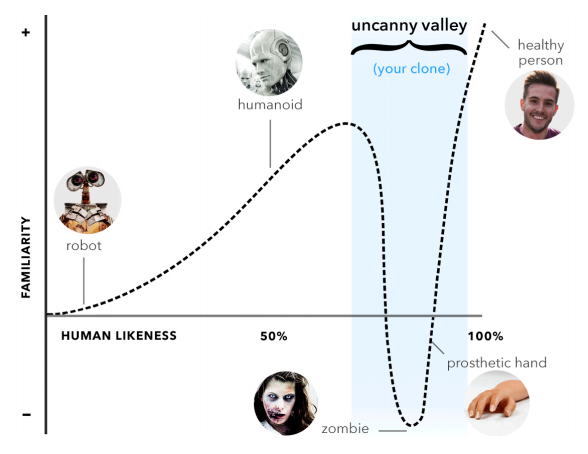
\includegraphics[scale=0.55]{./images/uncanny.png}
}
\end{figure}

\subsubsection{Actions}

On peut distinguer des actions basiques (move, jump, shoot) d\'efinis dans l'interface du jeu et les actions strat\'egiques qui sont dans le model mental du joueur (protect, sacrifice, pretend). Un jeu est \'el\'egant si un petit nombre d'actions de base autorise un grand nombre d'actions strat\'egiques ("emergent gameplay") .

\subsubsection{R\`egles}

On peut classifier les r\`egles du jeu de al fa\c{c}on suivante:

\begin{itemize}
\item Faisable: qui peut faire quelle action sur quel objet \`a quel moment? Example: Tu ne peux pas tirer qunad tu n'a pas assez d'\'energie.
\item Souhaitable: commet les actions d\'eterminent ma performance (score, victoire)? Exemple: un ligne \'elimin\'ee vaut 10 points, 2 lignes 50 points et 3 lignes 100 points.
\item R\`egle fondamentale ou objectif du joueur. Exemple: le but du jeu est d'\'eliminer tous les pingouins.
\end{itemize}

\subsubsection{Modes}

Des r\`egles diff\'erentes s'appliquent pendant diff\'erentes phases du jeu.

\begin{itemize}
\item Faisable: tu ne peux pas tirer quand tu n'a pas assez d'\'energie sauf en phase de tr\`eve.
\item Souhaitable: un ligne \'elimin\'ee vaut 10 points, 2 lignes 50 points et 3 lignes 100 points en mode collaboratif. Un ligne \'elimin\'ee vaut 30 points, 2 lignes 90 points et 3 lignes 300 points en mode comp\'etitif.
\end{itemize}

A chaque changement de mode, le joueur doit d\'esapprendre et r\'eapprendre. Alors,

\begin{itemize}
\item Le nombre de modes doit \^etre petit.
\item Le mode actif doit \^etre tr\`es visible pour l'utilisateur.
\end{itemize}

Une interface est "modale" si un m\^eme input produit diff\'erents effets selon le mode actif.

\begin{itemize}
\item Les modes permettent d'augmenter le nombre d'actions.
\item Le mode actif prend 1 slot en m\'emoire de travail.
\item Les interfaces "modeless" produisent moins d'erreur.
\end{itemize}

\subsubsection{Skills}

Il faut trouver un \'equilibre entre les skills du joueur et les skills de son personnage. 

Le joueur a des comp\'etences cognitives comme la m\'emoire, la d\'eduction, des connaissances, son raisonnement et son raisonnment spatial qui peuvent \^etre exploit\'e par des jeux diff\'erents. Ses comp\'etences physiques peuvent aussi \^etre exploit\'es. D'autres jeux ont un component de chance et finalment on peut m\'elanger les comp\'etences physiques et la chance.

\subsubsection{La chance}

Il faut alors trover un \'equilibre entre les skills du joueur et la chance qui va cr\'eer des surprises.

Bien que les ordinateurs ont une mauvaise r\'elation avec l'al\'eatoire, la pr\'sence d'un \^etre humain aux gestes physiques permet d'initier des ph\'enom\`enes pseudo-al\'eatoires.

\subsubsection{Points de vue ou position de la cam\'era}

Types de viewpoints:

\begin{itemize}
\item Cam\'era fixe: les objets (surtout personnages) sont rendus en temps r\'eel mais le d\'ecor est statique pendant une sc\`enes.
\item Top down: vue a\'erienne en 2D.
\item Scroll lat\'eral: la cam\'era se d\'eplace de gauche \`a droite avec le d\'eplacement de l'avatar.
\item Bird eye: vue \'elev\'ee en perspective depuis les yeux d'un oiseau.
\item First person: vue depuis les yeux de mon avatar.
\item over the shoulder: vue depuis l'\'epaule de l'interlocuteur de mon avatar.
\end{itemize}

La diff\'erence de point de vue est essentielle pour les jeux multi-players.

\begin{itemize}
\item Camer lock-on: la cam\'era doit suivre un ennemii.
\item Radar: vue de l'ensemble de l'espace, localisation du sous-espace actuellement affich\'e.
\item Contr\^olable: le joueur peut d\'ecider o\`u orienter son cam\'era.
\end{itemize}

\subsubsection{Vue}

Choisir la meilleure vue au meilleur moment constitue une comp\'etence-cl\'e dans le jeu.

\subsubsection{Roles}

Un role c'est la diff\'erente interaction des joueurs avec le jeu (gameplay assym\'etrique). Il est d\'efinit par un ensemble des r\`egles que chaque joueur doit respecter du sorte: "qui peut faire quelle action sur quel objet quand".

\subsubsection{Secrets}

D\`esigne qui et quand peut acc\`eder \`a l'information.

\subsubsection{Collaboration ou comp\'etition}

Les jeux collaboratives ou comp\'etitives sont \'etudi\'es en game theory.

\subsubsection{Mod\'elisation mutuelle}

Quels m\'ecanismes permettent au joueur A de pr\'edire ce que va faire le joueur B (\'equipier ou adversaire)?

Know ( John, Know (Mike, Know (John, treasure-location)))

On substitue la charge cognitive par la compilation par entra\^inement.

\subsubsection{Spectateurs}

La pr\'esence des spectateurs doit \^etre prise en compte dans le design du game mechanics.

\subsubsection{Triangularity}

On parle de triangularity quand on donne l'option au joueur d'obtenir peu de point pour un objetif facile et beaucoup des points pour un objectif difficile. 

\subsubsection{\'Echapper \`a la r\'ealit\'e}

\subsubsection{Scoreboard ou analytics}

\subsubsection{Gamification}

\textbf{Gamification}: is the application of game mechanisms to situations that aren't intrisically ludic.

All well designed games begin with a spirit of fun. Some games must deliver a serious and purposeful message, too. Unlike simple interactives, games have immediate feedback and require the player to accept rules on limited actions. \textbf{Serious Gaming} is used to teach and train K-12 students or as professional development. 

Games that blur the line between fun and education can all too frequently fall into the trap of becoming "edutainment," thinly disguised educational software or \textbf{"chocolate-covered broccoli"}. A coating of sweet does not make the learning suddenly fun. While no one expects a learning game to be on par with a blockbuster AAA title, like Battlefield 4, there should be no excuse for poor design. When reviewing Serious Game titles, look for ones that involve game mechanics common in entertainment games, like decision making, problem solving and role playing.

\subsubsection{Le flow}

Le "flow" (Mih\'aly Cs\'ikszentmih\'alyi) d\'ecrive l'\'etat mental d'une personne totalement "prise dans le jeu", immerg\'ee dans ce qu'elle fait, et qui fait preuve de:

\begin{itemize}
\item Une concentration totale sur un objet limit\'e.
\item Une perte de conscience de soi et de la notion du temps.
\item Setiement de contro\^ole de la situation.
\end{itemize}

Cet \'etat n\'ecessite:

\begin{itemize}
\item Objectifs clairs et des r\`egles.
\item Un feedback imm\'ediat.
\item Equilibre entre difficult\'e et comp\'etence.
\end{itemize}

\begin{figure}[H]
\centering
\makebox[\textwidth][c]{
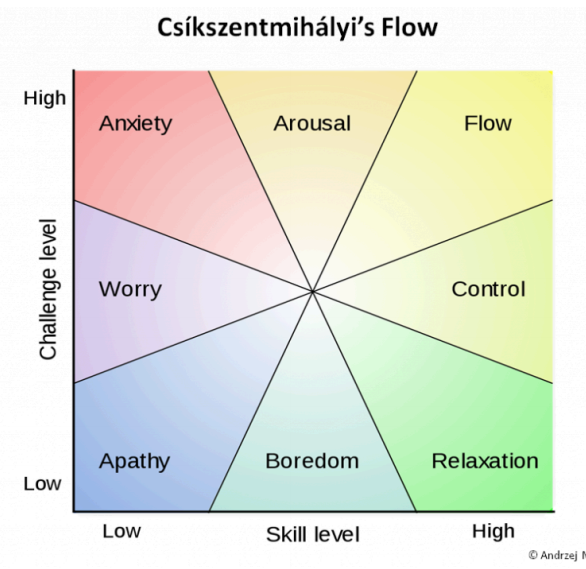
\includegraphics[scale=0.55]{./images/flow.png}
}
\end{figure}

\subsubsection{Motivation}

\textbf{Intrinsic motivation} (eviter la honte, chercher plaisir) refers to behavior that is driven by internal rewards. In other words, the motivation to engage in a behavior arises from within the individual because it is intrinsically rewarding. This contrasts with \textbf{extrinsic motivation} (eviter punition, chercher recompense), which involves engaging in a behavior in order to earn external rewards or avoid punishments.

\subsubsection{Exercises}

\begin{figure}[H]
\centering
\makebox[\textwidth][c]{
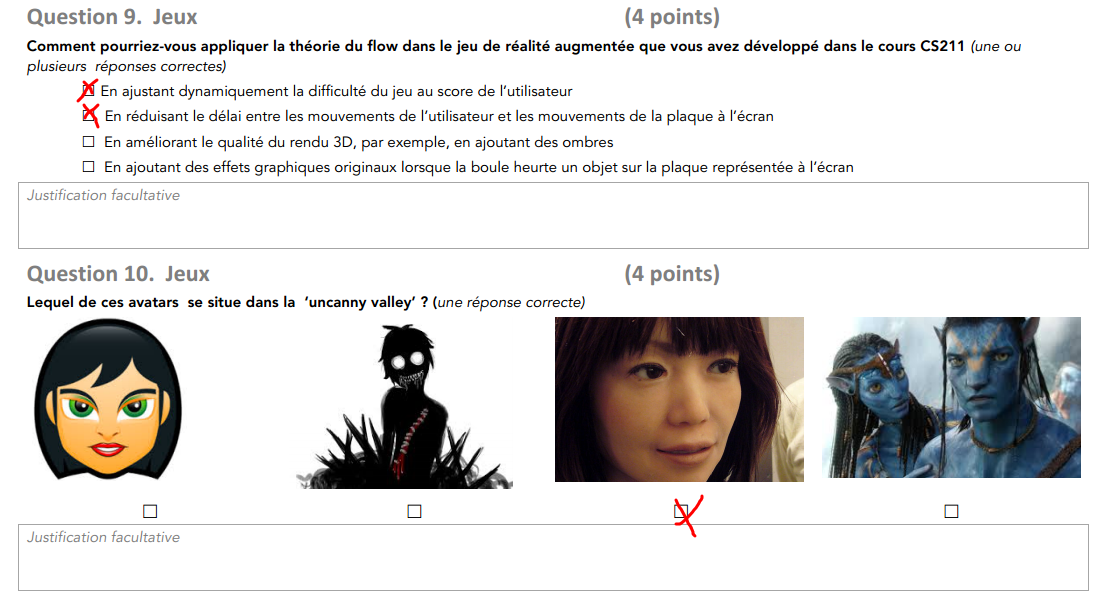
\includegraphics[scale=0.55]{./images/exercise2.png}
}
\end{figure}




\section{Usability}
Usability is the degree to which a software can be used by specified consumers to achieve quantified objectives with effectiveness, efficiency, and satisfaction in a quantified context of use.

\subsection{Comment savoir si l'interface est bien con\c{c}ue?}

Parmi tous les principes deux sont sp\'ecialement important: les utilisateurs sont efficaces et on a suivi les \textbf{principes du design}.

\subsubsection{8 golden rules de Ben Schneiderman}
\begin{itemize}
\item \textbf{Strive for consistency}: Utiliser les m\^emes interactions et termes dans les m\^emes situations. C'est difficile si on d\'eveloppe seul, mais si on d\'eveloppe en \'equipe, c'est impossible. Il faut des guidelines strictes.
\item \textbf{Enable frequent users to use shortcuts} (addr\'ess\'e aux experts).
\item \textbf{Offer informative feedback}: tel que "erreur possible", "en cours de traitement". Ici, on inclu le micro-feedback tel que "action possible" accompagn\'e du changement de curseur et de couleur du bouton ou "action per\c{c}ue" accompagn\'e du changement de couleur du bouton et d'un son "click".
\item \textbf{Design dialog to yield closure} (final de l'action).
\item \textbf{Offer simple error handling}: expliquer l'erreur et comment le r\'eparer. Aussi, pr\'evenir l'erreur.
\item \textbf{Permit easy reversal of actions}: "back", "cancel", "undo", "undo history", "revert".
\item \textbf{Support internal locus of control}: we want to make sure the user feels in control of the software and confident in how to accomplish their tasks.  A user should never be wondering “How did I get to this screen?” or “What do I need to press to do my task?” Navigation and task activation should always be clear and well-marked.
\item \textbf{Reduce short-term memory load}: don’t make your user remember more things than necessary.  If your system has information scattered across different screens that are needed for one task, consolidate those screens.  If a user enters information into a form, don’t make them re-enter it during a validation sequence.
\end{itemize}

\subsubsection{10 usability heuristics de Jakob Nielsen}

\begin{itemize}
\item Visibility of system status: par exemple avec un status bar.
\item Match between system and the real world: par exemple, on doit voir si la structure du site web refl\`ete la structure de l'entreprise qu'il pr\'esente ou la structure des besoins des utilisateurs.
\item User control and freedom.
\item Consistency and standards. 
\item Error prevention. 
\item Recognition rather than recall (cognitive load) 
\item Flexibility and efficiency of use (shortcuts)
\item Aesthetic and minimalist design
\item Help users recognize, diagnose, and recover from errors
\item Help and documentation
\end{itemize}

\subsubsection{6 design principles de Don Norman}

\begin{itemize}
\item Consistency: D\'etecter et appliquer des patterns
\item Visibility: Toutes mes actions possibles sont visibles
\item \textbf{Affordance}: la forme de l'objet nous indique comment l'utiliser
\item \textbf{Mapping}: le lien entre l'action et son effet sont \'evidents
\item Feedback
\item \textbf{Constraints}:  Interfaces must be designed with restrictions so that the system can never enter into an invalid state. Constraints, or restrictions, prevent invalid data from being entered and prevent invalid actions from being performed.
\end{itemize}

\subsubsection{Deux probl\`emes}

1. Les principes sont partiellement contradictoires

Montrer toutes les
optiosn possibles
Minimiser
l’information à
l’écran
Montrer toutes les options
probablement intéressantes

2. Les principes ne sont pas des solutions

Pour rédiger un bon résumé, il faut qu’il...
soit bref mais capture les points importants
soit général mais fournisse quelques détails
soit objectif mais doté d’un certain caractère
révèle l’essentiel mais donne envir de lire
...

\subsubsection{La solution}

La solution passe par des principes de design qui inspirent des prototypes qui son test\'es par les utilisateurs, un proc\'ess qui peut boucler.

\subsubsection{Prototypage}

La phase de prototypage peut obtenir diff\'erents d\'egr\'es de fid\'elit\'e. Nous n'aurions pas la m\^eme fid\'elit\'e en papier qu'avec des outils informatiques. 

The Wizard of Oz method is a research experiment in which participants use a computer system that is actually being operated or partially operated by an unseen user. This unseen user is known as the “wizard”. The purpose of the “wizard” is to simulate the actions of the program in real time while watching the user in the other room through a video feed. Users are often unaware that the software is not operative. This technique is good for testing device concepts and techniques, however it requires more equipment and planning.

\subsubsection{Testing}

On peut mesurer diff\'erent aspects dans le "usability":

\begin{itemize}
\item Learnability: combien de temps un novice a-t-il besoin pour manipuler le logiciel (NO USER GUIDE)?
\item Efficiency: combien de temps est n\'ecessaire pour faire la t\^ache qu'il veut faire?
\item Memorability: si ils ne l'utilisent pas pendant un certain temps, est-ce que c'est difficile d'y revenir?
\item Errors: Combien d'erreurs? Pr\^etent-elles \`a cons\'equence?
\item Satisfaction: Est-ce agr\'eable d'utiliser l'application?
\end{itemize}

Les phases pour tester l'application sont:

\begin{itemize}
\item Apprendre l'application
\item Pr\'eparer une liste de t\^aches
\item Recruter 8 utilisateurs (\'echantillon stratif\'e) (1 jour)
\item Leur demander de faire la t\^ache en pensant \`a voix haute, prendre note voir et enregistrer (1  jour)
\item (Leur demander ce qu'ils pensent)
\item Analyser les r\'esultats
\item Convaincre les concepteurs (1 jour)
\end{itemize}

\begin{itemize}
\item Le testeur n'est pas le d\'eveloppeur
\item Le testeur est ind\'ependant du d\'eveloppeur
\item Le d\'eveloppeur n'est pas pr\'esent
\item Le d\'eveloppeur vous d\'eniera
\end{itemize}

\subsection{Comment savoir si une interface de type X est plus efficace que une interface de type Y?}

Nous allons concevoir une exp\'erience pour savoir si une interface tangible permet de mieux jouer qu'un joystick. La variable ind\'ependante est alors l'input device (joystick ou interface tangible) et les variables d\'ependantes peuvent \^etre le score, la vitesse, le nombre d'erreurs, l'apprentissage, le plaisir ou la long\'etivit\'e. Le but de l'exp\'erience c'est de mesurer si les variations la variable ind\'ependante produisent des variations dans la variable d\'ependante.

On peut d\'esigner une exp\'erience \textbf{"between subjects"} c'est \`a dire, on forme deux groupes des personnes pour tester chacune des modalit\'es de la variable ind\'ependente. Un groupe et le groupe c\^ontrole qui ne se voit pas affect\'e par la variable ind\'ependante \'etudi\'ee et l'autre est le group exp\'erimental qui se voit affect\'e par la variable ind\'ependante.

On peut d\'esigner une exp\'erience \textbf{"within subjects"} o\`u les personnes dans la premi\`ere condition passent ensuite dans la deuxi\`eme. Pour contre-balancer l'effet d'ordre on inverse l'ordre de passage des deux conditions pour la moiti\'e des sujets. Dans cette modalit\'e on a besoin alors de la moiti\'e des sujets et les sujets sont id\'entiques dans les deux conditions. Mais les effets de l'ordre sont souvent assez compliqu\'es \`a interpr\'eter. 

L'exp\'erience peut tester aussi des autres variables ind\'ependantes: le type de jeu, le niveau des joueurs, la r\'esolution spatiale du logiciel ou \c{c}a vitesse. 

Prennons par example l'input device et le niveau comme variable ind\'ependante, alors on aurait six groupes pour la m\'ethode "between subjects". Dans cette situation il est possible que l'effet de la pr\'emi\`ere variable ind\'ependante sur la variable d\'ependante affecte la valeur de la deuxi\`eme variable ind\'ependante. Si on a une variable continue et une variable discr\`ete, une manque de d\'ependance entre les variables est visible par le parall\'ellisme des graphes dans la variable discr\`ete. 

On peut m\^eme avoir une troisi\`eme dimension. Avoir plus de deux dimensions pose des probl\`emes. Ainsi, pour N facteurs et M modalit\'es par facteur, on devrait avoir $M^N \cdot 20$ sujets. Les r\'esultats d'un tel exp\'erience sont aussi difficiles \`a interpr\'eter. Pour solutionner ces probl\`emes on peut d\'ecomposer en exp\'eriences successives \`a un ou deux dimensions pour mieux estimer la sensitivit\'e des variables.

Concevoir l'exp\'erience repose sur des principes tr\`es simples mais se heurte \`a moult subtils biais exp\'erimentaux:

\begin{itemize}
\item Est-ce que les sujets soumis aux diff\'erentes conditions \'etaient vraiment \'equivalents au d\'epart?

On peut consid\'erer ici l'\^age, niveau socio-culturel, scolaire, connaissances pr\'ealables, intelligence, raisonnement spacial ou motivation. Ces aspects peuvent \^etre m\'esur\'es par des questionnaires, dans le recrutement, avec des tests et avec la quantit\'e qu'on paye par exemple.

\item Est-ce que les sujets \'etaient inform\'es du but de l'exp\'erience? Est-ce que l'exp\'erimentateur \'etait vraiment neutre?

Un effet curieux c'est \textbf{l'effet Hawthorne}. Le simple fait de participer \`a une exp\'erience a une conse\'quence importante en termes de motivation. Ce qui peut affecter aux r\'esultat de la m\^eme. Un autre effet est \textbf{l'effet Pygmalion}. La performance des sujets est fonction des attentes de l'experimentateur. Un exemple est quand les proffesseurs ont plus d'expectatives dans certains \'el\`eves que dans des autres. Les \'el\`eves qui sont consid\'er\'es comme plus productifs vont produire plus que les autres. C'est pour \c{c}a que cet effet re\c{c}oit le nom de proph\'etie auto-r\'ealisatrice. L'exp\'erience de conservation des liquides, id\'ee de Jean Piaget, essaye d'identifier \`a quel \^age un enfant d\'eveloppe la capacit\'e de d\'etecter qu'une quantit\'e est pr\'serv\'ee m\^eme si on change le conteneur en forme ou taille. Cette exp\'erience a \'et\'e critiqu\'ee parce qu'elle souffre des effets mention\'es avant. En conclusion, il est difficile de faire des m\'ethodes en "double-aveugle" o\`u ni le sujet, ni l'exp\'erimentateur ne savent que le traitement est utilis\'e.

\item Est-ce qu'un \'el\'ement non-controll\'e peut expliquer les variations de la variable d\'ependante?

Dans toute exp\'erience il y a un nombre des variables interm\'ediaires ou variables de processus (comme la fatigue, la pr\'ecision, hauteur, log files, eye tracking, interactions) qui peuvent affecter au r\'esultat final. On appelle \textbf{effet de m\'ediation} \`a la relation entre variable ind\'ependante et variable d\'ependante qui s'explique statistiquement par une autre variable. Ainsi, une correlation entre les variables ne signifie pas causalit\'e mais la cause peut \^etre cach\'e par une autre variable.

Un autre probl\'eme est d'\'etablir si les variations qu'on observe dans les diff\'erents exp\'eriments sont vraiment \textbf{diff\'erences significatives} ou sont plut\^ot d\^u \`a une mal chance lors de la s\'election des sujets. Une m\'ethode pour ne pas obtenir une moyenne extr\^eme c'est de augmenter la taille de l'\'echantillon. Pour d\'eterminer si les diff\'erences sont significatives on compare alors la diff\'erence entre moyennes et la dispersion des \'echantillons.

Finalment, la technique de meta-analyse, combine les resultats de diff\'erents \'etudes scientifiques  pour avoir une plus grande s\^ur\'et\'e statistique.
\end{itemize}

\begin{exercise}
We compared new software for meetings the standard meeting rooms.

We selected 20 teams of 5 subjects and 20 teams of 10 subjects, i.e. 300 subjects. The ratio of women and men was the same in both conditions. The average age was respectively 34.3 and 33.9 years old.

Results : The time spent to agree on a solution was in average shorter with the new software. The degree of satisfaction was higher with the new software for teams of 5 but it was lower for the teams of 10. Teams
with the software produce in average shorter utterances and  participation was more balanced.

Find out which are:

\begin{itemize}
\item The 2 independent variables?
\item The 2 dependent variables?
\item The 2 controlled variables?
\item The 2 intermediate/process variables?
\item The 4 conditions?
\item The main effect?
\item The interaction effect?
\item Within subjects or between subjects
\end{itemize}
\end{exercise}

\begin{itemize}
\item The independent variables were the use or not of the software and the number of subjects in the group. 
\item The dependent variables were the time spent to agree to a solution and the degree of satisfaction.
\item The controlled variables were the number of women and men and the age of the subjects.
\item The intermediate variables were the number of utterances and the participation.
\item The four conditions were as follows: group of 5 not using software, group of 5 using software, group of 10 not using software and group of 10 using software.
\item The main effect was an improvement in the time spent to agree in a solution and not significant in the satisfaction (since we average the effects in the different independent variables).
\item The number of members in the team and the use or not of the software had an interaction effect: the degree of satisfaction was higher with the new software for teams of 5 but it was lower for the teams of 10.
\item The experience was carried out within subjects since every team experimented the use or not of the new software.
\end{itemize}

\begin{figure}[H]
\centering
\makebox[\textwidth][c]{
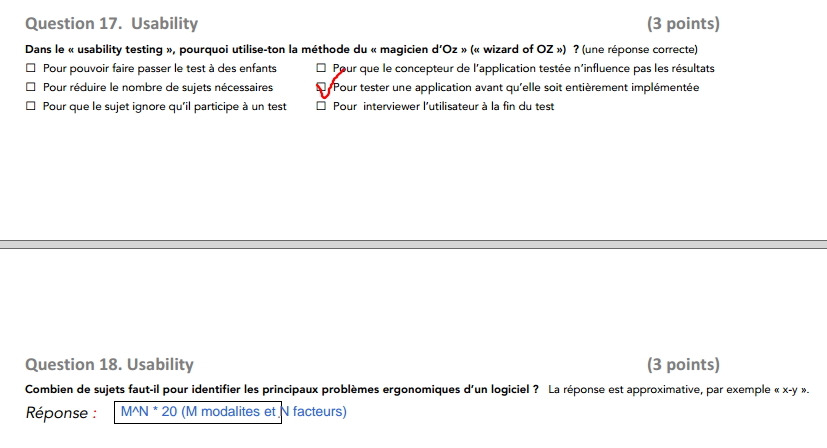
\includegraphics[scale=0.55]{./images/exercise4.png}
}
\end{figure}




































\end{document}
